\chapter{Introduction}
The Lead Radius Experiment-II (PREX-II) and the Calcium Radius Experiment (CREX) are high-precision experiments that measure the tiny parity-violating (PV) asymmetry at the parts-per-million (ppm) level. These experiments use longitudinally polarized electrons to scatter off neutron-rich targets such as \Pb and \Ca, allowing for the extraction of weak form factor, weak charge, neutron distribution, and the neutron skin thickness of the target nucleus.

The PV asymmetry ($\CA_{\text{PV}}$) arises due to the interference between the electromagnetic (EM) and neutral weak one-boson exchange amplitudes, as weak interactions violate parity. As the EM interaction has been well-understood, the PV asymmetry measurement enables the extraction of the weak charge, and consequently, the distribution of the neutron (which carries almost all of the weak charge) inside a nucleus.

Parity-violating electron scattering (PVES) experiments require a longitudinally polarized electron beam of high quality, which was provided by the Continuous Electron Beam Accelerator Facility (CEBAF) at Thomas Jefferson National Accelerator Facility (TJNAF, also known as JLab) for PREX-II and CREX experiments. The excellent beam quality and dedicated instrumentation at JLab allowed for statistics-limited asymmetry measurements.

% physical implication
% 1. neutron distribution
%%%%%%%%%%%%%%%%%%%%%%%%%%%%%%%%%%%%%%%%%%%%%%%%%%%%%%%%%%%%%%%%%%%%%%%%
\section{Point-Neutron Radius and Neutron Skin}
Despite the advances in modern physics, we still lack a clear way to compute the size of a nucleus, and we may not even fully understand what we mean by ``size''. In a simple model, one can estimate the nuclear radius as $R = R_0 A^{1/3}$, where $A$ is the nuclear mass number and $R_0$ is an experimentally determined constant ($R_0 \approx 1.20$~fm) \cite{ROYER2008105}. However, this model only works for spherical nuclei and fails for deformed nuclei. It is better to calculate the radius of a nucleus from its nucleon density distribution, treating the nucleons as point particles. Physicists have successfully calculated and precisely measured the point-proton radii of many nuclei \cite{DEVRIES1987495, ANGELI201369}. However, the neutron, being neutral, poses a significant challenge to measuring the inner structure of nuclei. This is especially true for heavy nuclei, where more neutrons than protons are needed to bind the nucleus. In such cases, it is the point-neutron radius(referred to hereafter as simply the neutron radius), rather than the point-proton radius (proton radius), that dominates the size of the nucleus.

When discussing the proton or neutron radius, we are referring to a concept within the framework of quantum mechanics (QM) rather than classical mechanics. In QM, a particle is described by a wave function, and the square of its normalized magnitude corresponds to the probability of finding the particle in a specific state. Therefore, the proton (neutron) root-mean-square (RMS) radius is defined as:
% why RMS radius, rather than r\rho(r) directly?
\begin{equation}
    R_{p, n} \equiv \langle R_{p,n}^2\rangle^{1/2} = \sqrt{\frac{\int d^3\vec{r}\,r^2\,\rho_{p,n}(\vec{r})}{\int d^3\vec{r}\,\rho_{p,n}(\vec{r})}}
    \label{eq:nucleon_rms_radius}
\end{equation}
where $\rho(\vec{r})$ is the normalized proton (neutron) density at position $\vec{r}$.
\begin{equation}
    \int d^3\vec{r} \rho_{p, n}(\vec{r}) = 1 
\end{equation}

There are numerous papers in the literature reporting high-precision measurements
(with an uncertainty at the $0.01$~fm level) of the proton radius ($R_p$, also called
the charge radius) of various nuclei through atomic and nuclear experiments \cite{DEVRIES1987495, ANGELI201369}. 
In contrast, determining the neutron radius ($R_n$) precisely is more challenging 
due to the neutron's lack of electric charge. This means its size can only be 
measured through strong or weak interactions, and both of which suffer from their limitations.

The weak interaction has a coupling constant ($\alpha_W$) between $10^{-7}$ and $10^{-6}$ \cite{hyperphysics}, which is much weaker than the electromagnetic coupling constant ($\alpha$) of about $10^{-2}$. As a result, it is difficult to control systematic uncertainties if measured directly. To overcome this challenge, scientists have turned to the measurement of the parity-violating (PV) asymmetry. By taking the asymmetry between two electron beams with opposite helicities, many systematic uncertainties can be cancelled, leading to high precision measurements.

In terms of the strong interaction, the effective coupling has large theoretical uncertainties rooted 
in the non-perturbative nature of the underlying quantum chromodynamics (QCD) at low energy scale.
Therefore, interpreting hadronic measurements often relies on theoretical models, leading to model-dependent results.

Despite the many challenges involved, there has been significant effort and progress from 
the scientific community to explore different aspects of the neutron radius (and neutron skin thickness).
Hadronic probes, including pion \cite{ALLARDYCE19731}, proton \cite{LOMBARDI1972103,PhysRevC.82.044611}, 
antiproton \cite{PhysRevC.76.014311} and alpha particle \cite{KRASZNAHORKAY2004224},
as well as atomic experiments such as electric dipole polarizabilities \cite{Roca_Maza_2012} and 
pygmy dipole resonances \cite{PhysRevC.88.044610}, provide valuable inputs to our understanding.
Currently, experimental measurements of $R_n$ have a resolution of better than 1\%.
On the theory side, the most precise estimate of $R_n$ comes from nuclear models
that have been constrained primarily by data other than measurements	% FIXME reference
of neutron radii. Therefore, a precise measurement of $R_n$ would provide a powerful 
independent check of the basic nuclear theory.
\begin{comment}
% https://doi.org/10.1016/j.nuclphysa.2003.11.034
\item proton
    \begin{itemize}
	\item high-energy polarized proton
	\item Relativistic Impulse Approximation (RIA) with free nucleon-nucleon interaction
    \end{itemize}
\item pion
    \begin{itemize}
	\item in the $\Delta(1332)$ region, $\pi^- N$ interaction is 3 times larger than $\pi^- p$.
	\item strong absorption at the surface, sensitive to the tail of neutron distributions;
	    increase pion energy to reduce cross section
	\item applicable to only light stable nuclei
    \end{itemize}
\item antiproton
    \begin{itemize}
	\item slow antiproton capture (like an electron)
    \end{itemize}
\item PVES
\item GDR: Giant Dipole Resonance
\item SDR: Spin-Dipole Resonance
\end{comment}

Experimentally, the nucleon radius is obtained from the corresponding form
factors (FFs). In QM, under the Born approximation, the matrix element (ME) 
for the scattering of a plane wave (a free particle) from a Coulomb-like potential 
(a target nucleus) is:
\begin{equation}
    \begin{aligned}
	\CM_{fi} &= \bra{\Psi_f}V(\vec{r})\ket{\Psi_i} 
		= \int e^{-i\vec{p}_f\vec{r}}V(\vec{r}) e^{i\vec{p}_i\vec{r}} d^3\vec{r}    \\	% 1
	    &= \int e^{i(\vec{p_i} - \vec{p_f})\vec{r}} d^3\vec{r} 
		\int \frac{Q_t\rho(\vec{r'})}{4\pi|\vec{r} - \vec{r'}|} d^3\vec{r'} \\	% 2
	    &= \int \int e^{i\vec{q} \vec{r} } 
		 \frac{Q_t \rho(\vec{r'})}{4\pi|\vec{r} - \vec{r'}|} d^3\vec{r} d^3\vec{r'} \\	% 2
	    &= \int\int e^{i\vec{q}(\vec{r} - \vec{r'})} 
		\frac{Q_t\rho(\vec{r'})}{4\pi|\vec{r} - \vec{r'}|} e^{i\vec{q}\vec{r'}} d^3\vec{r} d^3\vec{r'}   \\  % 3
	    &= \int e^{i\vec{q}\vec{R}} \frac{Q_t}{4\pi|\vec{R}|} d^3\vec{R} 
		\int \rho(\vec{r'}) e^{i\vec{q} \vec{r'}}d^3 \vec{r'}	\\  % 4
	    &= (\CM_{fi})_{\text{Mott}} F(\vec{q})   \\	% 5
    \end{aligned}
    \label{eq:ME}
\end{equation}
where $\vec{p}_i$ and $\vec{p}_f$ denote momentum of the incoming and outgoing particles respectively,
and $\vec{q} = \vec{p}_i - \vec{p}_f$ refers to the momentum transfer during the scattering,
while $Q_t$ represents the total charge of the target nucleus. The ME can be factorized into two parts:
the amplitude of a Mott scattering, which describes the scattering of a particle from 
a point-like nucleus with charge $Q_t$, and a modification
due to the inner structure of the target nucleus, known as the FF:
\begin{equation}
    F(\vec{q}) = \int \rho(\vec{r}) e^{i\vec{q} \vec{r}} d^3\vec{r}
    \label{eq:ff}
\end{equation}
The FF is the Fourier transform of the spatial density distribution.
Conversely, once the FFs at different $\vec{q}$ are konwn or measured, 
the charge distribution can be derived:
\begin{equation}
    \rho(\vec{r}) = \int F(\vec{q}) e^{-i\vec{q}\vec{r}} d^3\vec{q}
\end{equation}
What is more, $F(\vec{q})$ can be experimentally measured, as shown in Eq.~\ref{eq:ME}:
\begin{equation}
    F(\vec{q}) = \frac{\CM_{fi}}{(\CM_{fi})_{\text{Mott}}} 
	= \sqrt{\frac{\sigma_{\text{measured}}}{\sigma_{\text{Mott}}}} 
\end{equation}
The problem is, experimentally, it is not feasible to cover the entire phase space 
of $\vec{q}$, and therefore, only a limited number of data points at selected $\vec{q}$ 
can be measured. Consequently, phenomenological models are required to extract the charge density distribution. 
% FIXME: examples of phenomenological models

For a spherically symmetric density distribution, 
$\rho(\vec{r}) = \rho({|\vec{r}|}) = \rho(r)$, 
the corresponding FF is calculated as:
\begin{equation}
    F(\vec{q}) = \int \rho(r) e^{iqr\cos\theta} 2\pi r^2 \sin\theta dr d\theta
	= 4\pi \int r \rho(r) \frac{\sin{(qr)}}{q} dr
    \label{eq:spherically_symmetric_FF}
\end{equation}
One can observe that for a Coulomb-like potential, $F(\vec{q})$ does not depend on
the direction of $\vec{q}$, but solely on its magnitude: $q$. For the sake 
of Lorentz invariance, $F$ is usually expressed in terms of $Q^2 = -q^2$, rather
than $q$. Therefore, we will use $F(q^2)$ or $F(Q^2)$ in the following discussions.

Some typical spherically symmetric density distributions and their 
corresponding FFs are shown in Fig.~\ref{fig:FFs}.
\begin{figure}[!h]
    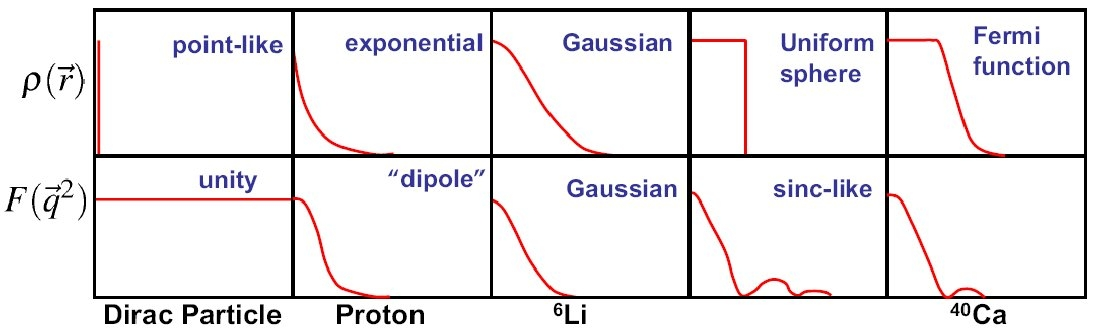
\includegraphics[width=0.9\linewidth]{rho_vs_FF}
    \caption{Characteristic of FFs w.r.t. different density distribution functions}
    \label{fig:FFs}
\end{figure}

In the small $\vec{q}^2$ limit ($q^2 << 1$), one can perform a Fourier expansion on both
sides of Eq.~\ref{eq:spherically_symmetric_FF}:
\begin{equation}
    F(q^2) = F(0) + \left.\frac{dF}{dq^2}\right|_{q^2=0} \times q^2 + \cdots	\\
    \label{eq:FF_FE_1}
\end{equation}
\begin{equation}
    \begin{aligned}
	F(q^2) &= 4\pi \int r \rho(r) \frac{\sin{(qr)}}{q} dr \\
	    &= 4\pi \int \rho(r) r \left( r - \frac{1}{6} q^2r^3 + \cdots \right) dr	\\
	    &= \int \rho(r)  \left( 1 - \frac{1}{6} q^2r^2 + \cdots \right) 4\pi r^2 dr	\\
	    &= 1 - \frac{1}{6}q^2\langle R^2 \rangle + \cdots \\
    \end{aligned}
    \label{eq:FF_FE_2}
\end{equation}
Matching Eq.~\ref{eq:FF_FE_1} to \ref{eq:FF_FE_2} yields
\begin{equation}
    \langle R^2 \rangle = \int r^2 \rho(r) d^3\vec{r} = -6 \left. \frac{dF(q^2)}{dq^2} \right|_{q^2 = 0}
\end{equation}
This equation hints how to measure the RMS radius.
One can measure the FFs at several small $q^2$ points, extrapolate them 
to $q^2 = 0$, and then calculate the slope at $q^2 = 0$ to obtain the RMS radius.
\footnote{This is why we use the RMS radius rather than the more physically intuitive definition of: 
$\langle R \rangle = \int  r \rho(\vec{r}) d^3\vec{r}$.}

For electrically charged proton, the FF will be the precisely measured EM FF:
\begin{equation}
    \langle R_p^2 \rangle \approx \langle R_{ch}^2 \rangle= -6 \left. \frac{dF_{EM}(q^2)}{dq^2} \right|_{q^2 = 0}
\end{equation}
Since neutron is electrically neutral, its RMS radius will be measured from its weak charge FF:
\begin{equation}
    \langle R_n^2 \rangle \approx \langle R_W^2 \rangle = -6 \left. \frac{dF_{W}(q^2)}{dq^2} \right|_{q^2 = 0}
\end{equation}
The difference between the neutron and the proton RMS radii is referred to as the neutron skin thickness:
\begin{equation}
    R_{\text{skin}} = R_n - R_p = \sqrt{\langle R_n^2 \rangle} - \sqrt{\langle R_p^2 \rangle}
\end{equation}
a concept that was first suggested by Johnson and Teller \cite{PhysRev.93.357}
and first observed in the $K^-$ meson capture processes \cite{BURHOP1969625}.

The neutron skin is founded in neutron-rich atomic nuclei that contain more
neutrons than protons. Analogous to the atomic electron shell model, the nuclear
shell model proposes that protons and neutrons also arrange themselves in
shells from low to high energy levels without disturbing each other.
The higher the energy level, the larger the orbital radius.
For symmetric nuclei, we expect similar neutron radii to proton radii. 
However, in neutron-rich nuclei, the extra neutrons must occupy 
higher energy orbits after filling all the low energy ones, resulting in
a larger radius than that of the proton, and therefore, the formation of a neutron skin.

The deep reason why these extra neutrons form a neutron skin instead of
a neutron core lies in the symmetry energy and its dependence on nucleon density. 
The symmetry energy represents the penalty for breaking the proton-neutron symmetry,
whose value increases with nucleon density \cite{10.3389/fphy.2019.00213}.
As the core has a higher nucleon density than the surface, the higher the density, 
the larger the symmetry energy, leading to a lower binding energy
\footnote{the energy needed to break down a bounded nuclear system: $BE(N, Z) = M(N, Z)c^2 - Zm_p c^2 - Nm_n c^2$}, 
and less stable nuclei. So it is the symmetry energy that pushes these extra neutrons to 
the surface. On the other hand, as the number of nucleons on the surface increases, 
so does the surface tension, which favors squeezing extra neutrons % FIXME reference for the surface tension
into the core. The balance between the symmetry energy and 
the surface tension determines the thickness of the neutron skin.

% FIXME: a conclusion paragraph stating the importance of the measurement

%%%%%%%%%%%%%%%%%%%%%%%%%%%%%%%%%%%%%%%%%%%%%%%
\subsection{Theoretical Models} 
\label{subsec:models}
Though we lack knowledge of the actual neutron distribution, it is reasonable to assume that protons and neutrons share the same distribution function, with only minor variations in function parameters, even in nuclei with asymmetric numbers of protons and neutrons. Hence, the proton distribution provides a good starting point for studying the neutron distribution, considering our comprehensive understanding of proton distribution through various eA and AA scatterings. The elastic scattering cross-section is described in \cite{punjabi2015structure}.
\begin{equation}
    \frac{d\sigma}{d\Omega} = \left( \frac{d\sigma}{d\Omega} \right)_{\text{Mott}} |F(q^2)|^2
\end{equation}

The FF encodes information about the charge distribution of a nucleus. It is an interference
effect: the finite size of the scattering center introduces a phase difference between
different plane waves scattered from different points in space.
\begin{figure}
    \centering
    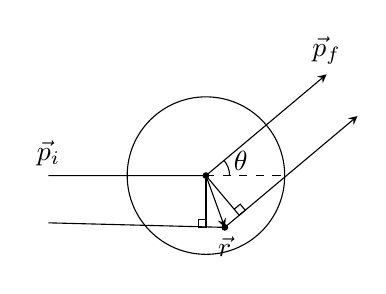
\begin{tikzpicture}
	% theta = 40, r = 0.7
	\coordinate (O) at (0, 0);
	\coordinate (P) at (-70:0.7);
	\draw (O) circle (1 cm);
	\draw[fill=black] (O) circle (1 pt);
	\draw[fill=black] (P) circle (1 pt);
	\draw[-stealth] (-2, 0) node [above] {$\vec{p}_i$} -- (O) -- ++(40:2) node [above, sloped] {$\vec{p}_f$};
	\draw[-stealth] (-2, -0.6) -- (P) -- ++(40:2.2);
	\draw[-stealth] (O) -- (P) node[below] {$\vec{r}$};
	\draw[dashed] (O) -- +(1, 0);
	\draw (0.3, 0) arc (0:40:0.3) node[right] {$\theta$};

	\draw (O) -- ++(0, -0.657785) -- ++(-0.1, 0) -- ++(0, 0.1) -- ++(0.1, 0);
	\draw (O) -- ++(-50:0.657785) -- ++(40:0.1) -- ++(130:0.1) -- ++(-140:0.1);
    \end{tikzpicture}
    \caption[eA scattering]{Schematic plot of eA scattering. As one can see, the wave scattered
    at position $\vec{r}$ will travel extra distance compared to the one scattered
    at the object center, which leads to a phase difference of:
    $\delta = e^{i[\vec{p}_i \cdot \vec{r} + (-\vec{p}_f) \cdot \vec{r}]} = e^{i\vec{q}\cdot\vec{r}}$.
    }
    \label{fig:FF_phase_diff}
\end{figure}

Consider a simple hard ball model:
\begin{equation}
    \rho(r) = 
    \begin{cases}
	\frac{3}{4\pi R^3}  & r \le R	\\
	0		    & r > R   \\
    \end{cases}
    \label{eq:hard_ball_model}
\end{equation}
Then the FF will be:
\begin{equation}
    F(q^2) = \frac{3}{(qR)^3} \left( \sin(qR) - qR\cos(qR) \right)
\end{equation}
where $q = 2p\sin(\theta/2)$.

Given the Mott cross section \cite{punjabi2015structure}: 
% \begin{equation}
%     \left( \frac{d\sigma}{d\Omega} \right)_{Mott} = 
%     \begin{cases}
% 	\frac{Z^2 \alpha^2}{4E^2\sin^4(\theta/2)}\cos^2(\theta/2)   
% 	    & \text{light nuclei} \ Z\alpha << 1  \\
% 	\frac{Z^2 \alpha^2}{4E^2\sin^4(\theta/2)}\cos^2(\theta/2) \left[ 1 + \pi Z \alpha \frac{\sin(\theta/2)(1-\sin(\theta/2)))}{\cos^2(\theta/2)}\right]   
% 	    & \text{medium nuclei}  \\
%     \end{cases}
% \end{equation}
\begin{equation}
    \left( \frac{d\sigma}{d\Omega} \right)_{\text{Mott}} = 
	\frac{Z^2 \alpha^2}{4E^2\sin^4(\theta/2)}\cos^2(\theta/2)   
\end{equation}
the resulting cross section, as a function of the scattering angle, is shown in Fig.~\ref{fig:ca_xsec}.
\begin{figure}
    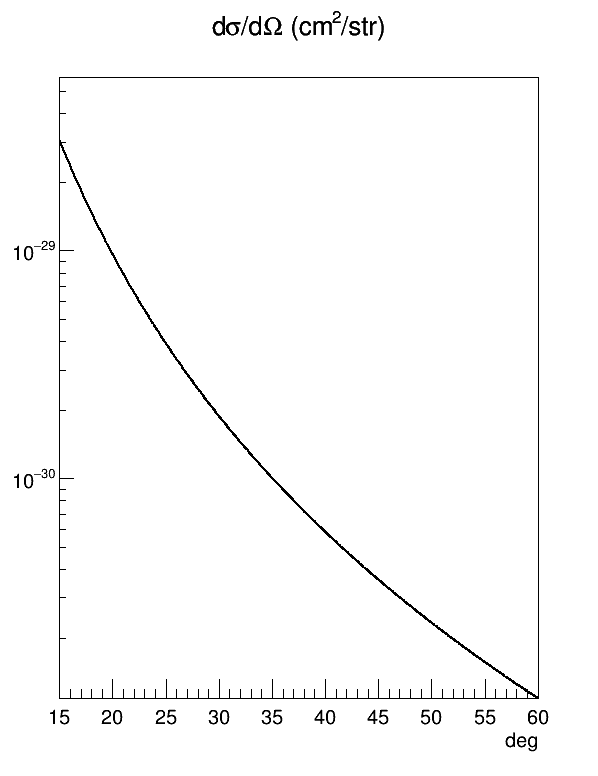
\includegraphics[width=0.32\linewidth]{ca48_xsec_mott}
    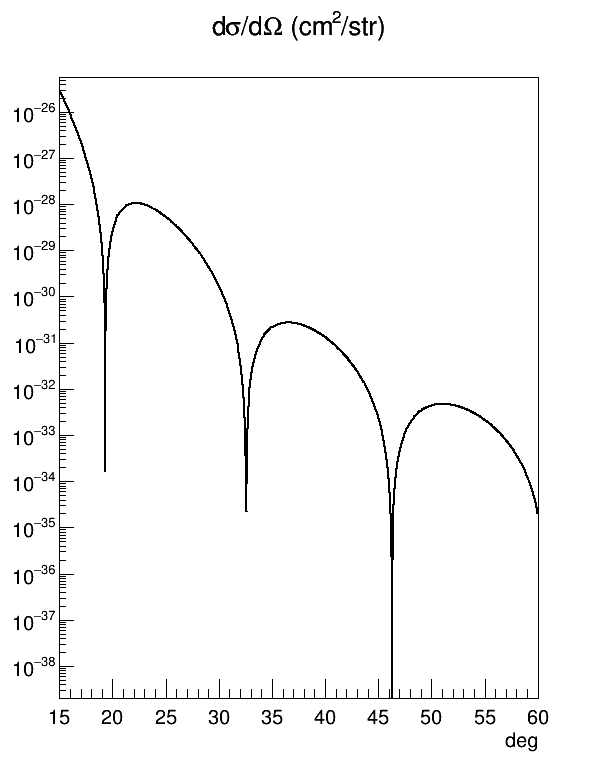
\includegraphics[width=0.32\linewidth]{ca48_xsec_hard_ball}
    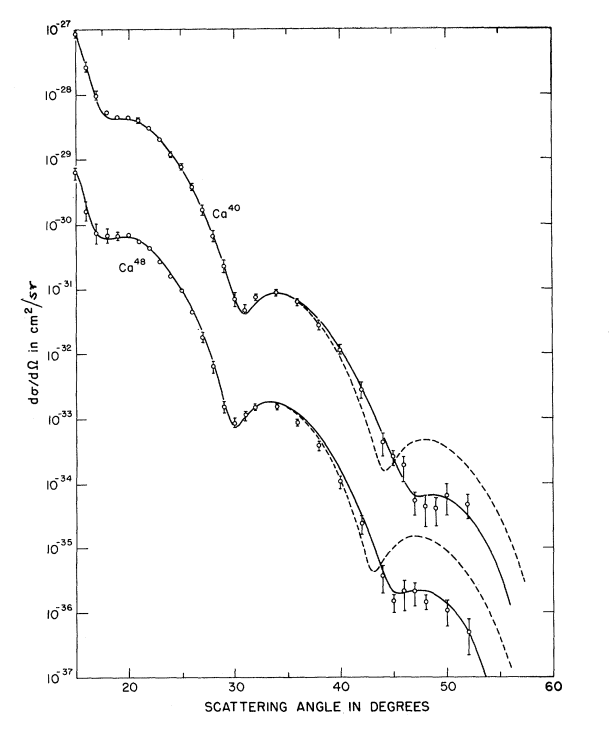
\includegraphics[width=0.32\linewidth]{ca_xsec_exp}
    \caption[Cross section of \Ca]{Left: Mott cross section for electron elastically scattered off a \Ca
    target with parameters: $p=E=757.5$~MeV.
    Middle: cross section for electron elastically scattered off Ca48 with the hard ball
    model (\ref{eq:hard_ball_model}) with parameters: $E =  757.5$~MeV, $R=A^{1/3}$~fm. 
    Right: experimental values (dots) and theoretical prediction (solid line)
    assuming the charge distribution as a three-parameter Fermi function (\ref{eq:3-para_Fermi}).
    for \Ca \ (\ca) targets, which are multiplied by $10^{-1}$ ($10$) to differentiate them
    \cite{PhysRevLett.19.527}. A similar cross section plot for \Pb can be found
    in \cite{PhysRevLett.38.152}.
    }
    \label{fig:ca_xsec}
\end{figure}

While the hard ball model does not reproduce the experimental distribution, it does
characterize the real distribution and demonstrate how the FF modifies the cross section:
the oscillating dips. A more realistic model for the density distribution is the
Woods-Saxon distribution (also known as the Fermi two-parameter model or the Fermi
distribution):
\begin{equation}
    \rho(r) = \frac{\rho(0)}{1 + \exp((r-R)/t)}
\end{equation}
where $R = (1.2A^{1/3} - 0.48)$~fm denotes the nuclear force radius at which 
$\rho(r) = \frac{\rho(0)}{2}$. The parameter $t$, which is typically in
the range of $0.4-0.5$~fm for  $A > 40$, indicates the surface thickness, 
over which $\rho(r)$ falls from 90\% to 10\%.
\begin{figure}[!h]
    \centering
    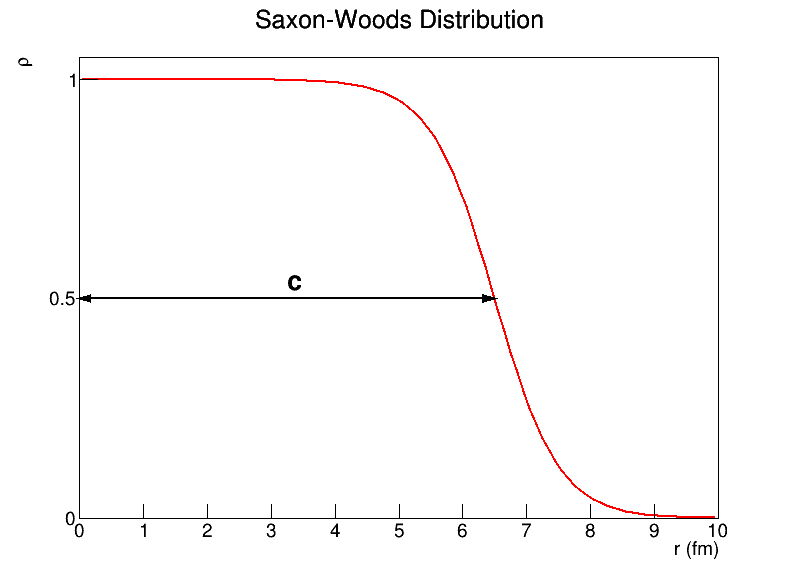
\includegraphics[width=0.5\linewidth]{fermi_distribution}
    \caption[fermi distribution]
    {In the nuclear shell model, it is assumed that nucleons occupy 
    different eigenstates of the same spherically symmetric average potential.
    However, unlike in the atomic shell model, this potential must be guessed. 
    It turns out that the Woods-Saxon model is a good candidate for this potential: 
    $V(r) = -\frac{V(0)}{1+\exp((r-c)/a)}$ ($c$ is the half-height radius and $a$ represents
    diffuseness of the distribution). This potential is formed
    by all other nucleons and is approximately proportional to the nucleon density, 
    therefore the same distribution for nucleon density.} 
\end{figure}

Fig.~\ref{fig:ca_xsec} (right) uses a fine tuned three-parameter Fermi function:
\begin{equation}
    \rho(r) = \frac{\rho_0(1 + \omega r^2/R^2)}{1 + \exp((r-R)/t)}
    \label{eq:3-para_Fermi}
\end{equation}
the central depression parameter $\omega$ allows the central density to be depressed
or raised, depending on the sign of $\omega$. More detailed discussion about the Fermi 
distribution can be found in \cite{Maximon:1966sqn}.

One example model based on the Fermi distribution is the FSUGold \cite{PhysRevLett.95.122501},
the neutron distribution of \Pb predicted by FSUGold is shown in Fig.~\ref{fig:FSUGold_pb208}.
\begin{figure}[!h]
    \centering
    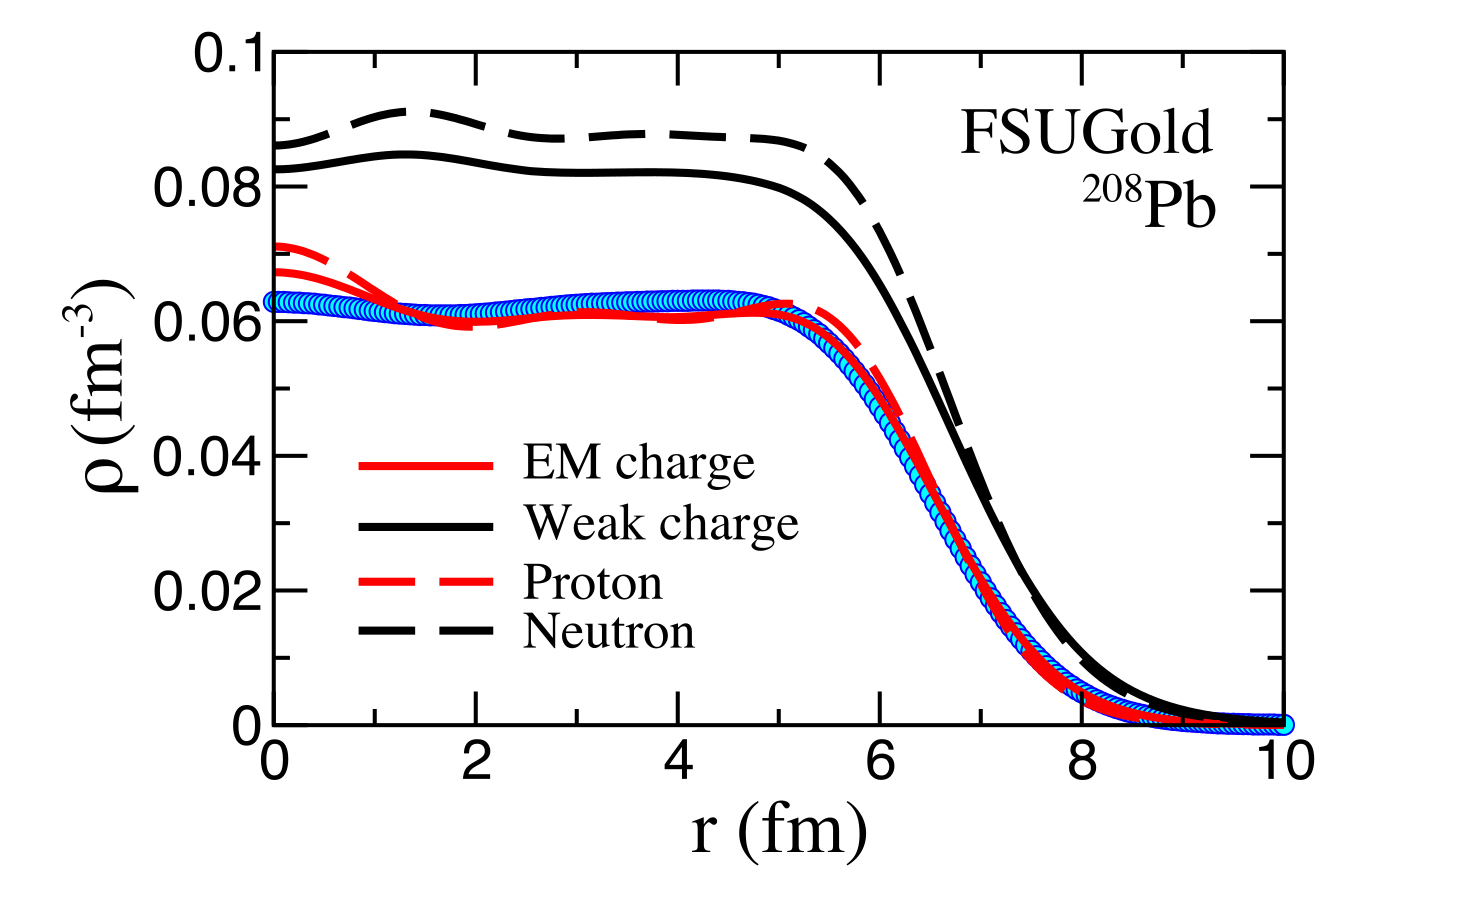
\includegraphics[width=0.6\linewidth]{FSUGold_pb208}
    \caption[Neutron distribution from FSUGold]
    {Neutron and weak charge distribution in \Pb predicted by the FSUGold model.
    The blue dots are experimental measurements of the charge distribution.}
    \label{fig:FSUGold_pb208}
\end{figure}

For medium and heavy nuclei, the Born approximation, which assumes that 
the incoming and outgoing waves are plane waves, is no longer valid.
Because the waves are distorted by the strong nuclear EM field. 
Therefore, the Coulomb distortion effect needs to be taken into account, 
which significantly modifies the PV asymmetry.

Coulomb distortion can be understood as multiple EM interactions with
the same nucleus, so the distortion correction is proportional to $Z\alpha$. 
This correction is particularly important for heavy nuclei like \Pb due to their
large Z values. Coulomb-distortion can reduce the PV asymmetry by as much as 30\%,
as shown in Fig.~\ref{fig:diff_by_Coulomb_distortion}.
\begin{figure}[H]
    \centering
    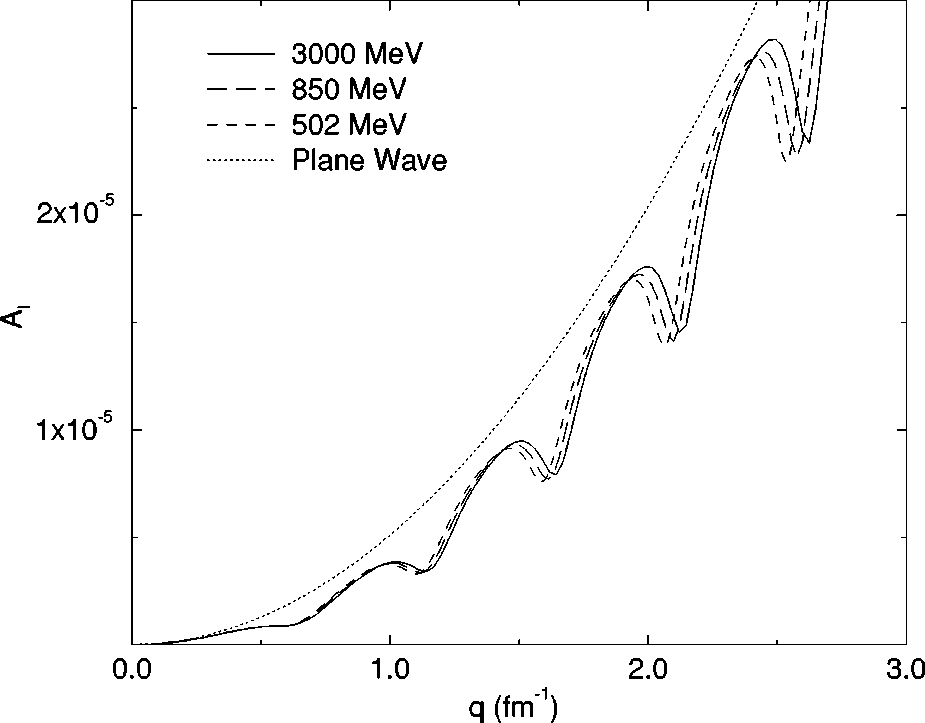
\includegraphics[width=0.5\linewidth]{Coulomb_distortion_Pb208_diff}
    \caption[Coulomb distortion]
    {Comparison of PV asymmetries with and without the effect of Coulomb
    distortion for \Pb. The calculation assumes the same weak and charge densities,
    which are taken to be the three-parameter Fermi function \cite{PhysRevC.57.3430}.
    }
    \label{fig:diff_by_Coulomb_distortion}
\end{figure}

With these information, one can solve the Dirac equation directly to obtain
the PV asymmetry, as illustrated in Fig.~\ref{fig:Coulomb_distortion}.

\begin{figure}[!h]
    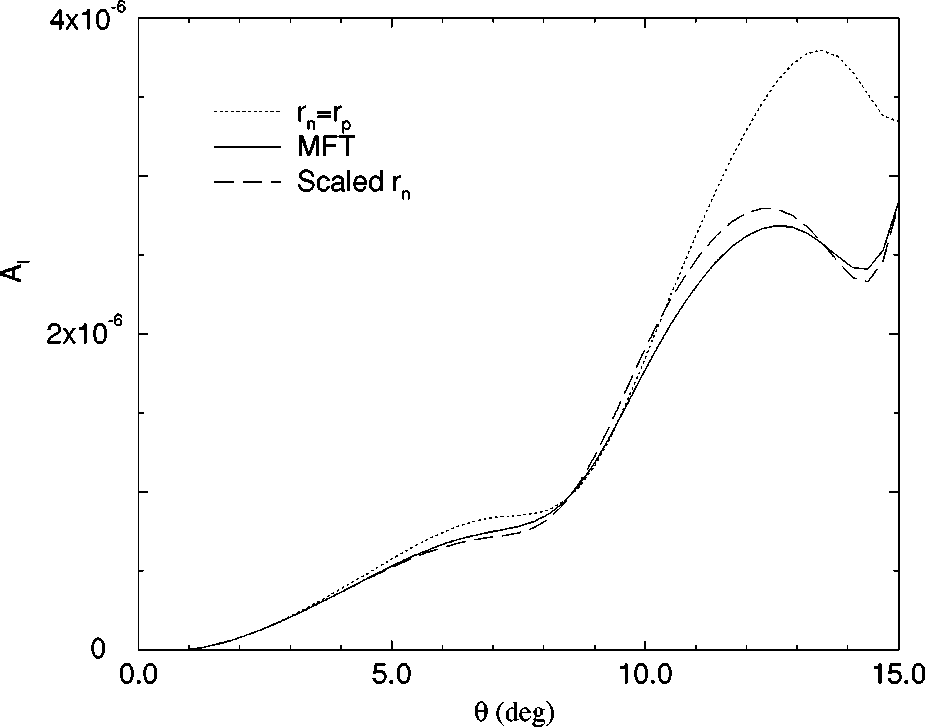
\includegraphics[width=0.49\linewidth]{Coulomb_distortion_Pb208}
    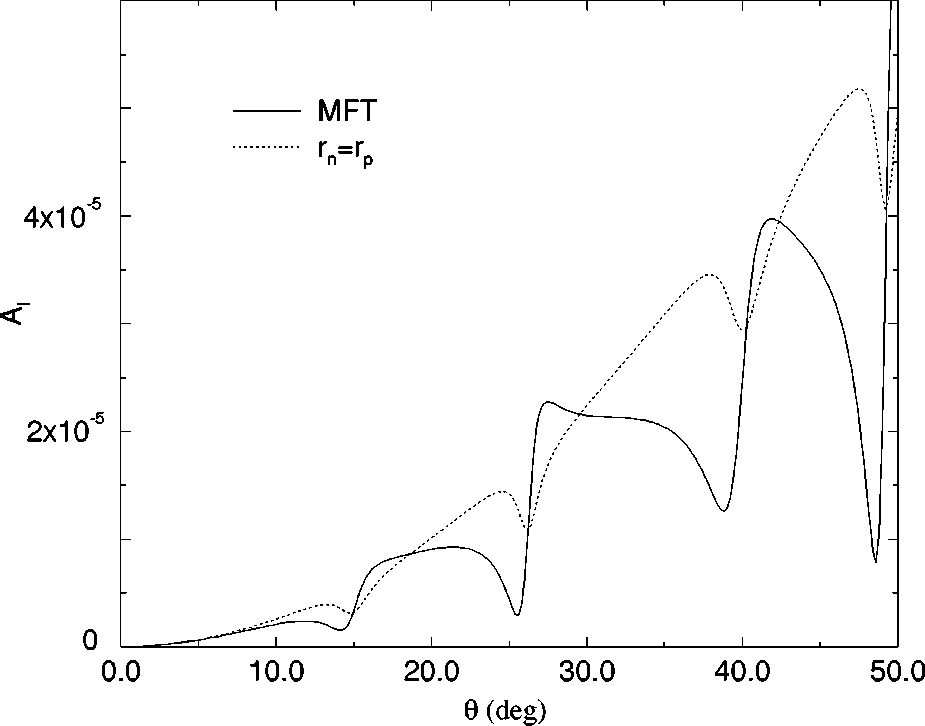
\includegraphics[width=0.48\linewidth]{Coulomb_distortion_Ca48}
    \caption[PV asymmetry for \Pb and \Ca]
    {PV asymmetry for \Pb (left) and \Ca (right) versus scattering angle 
    at 850~MeV, including the Coulomb distortion effect. 
    The dotted curve assumes the same weak and charge distributions (three-parameter Fermi function), 
    while the solid curve is based on relativistic mean field densities.
    The dashed curve uses a stretched density distribution based on the three-parameter Fermi function \cite{PhysRevC.57.3430}.
    }
    \label{fig:Coulomb_distortion}
\end{figure}

% 2. symmetry energy dependence on density
%%%%%%%%%%%%%%%%%%%%%%%%%%%%%%%%%%%%%%%%%%%%%%%%%%%%%%%%%%%%%%%%%%%%%%%%
\section{Symmetry Energy} 
The binding energy of a nuclear system depends on both the total number of nucleons ($A$),
and the difference between the numbers of protons and neutrons. To describe it,
we can use the liquid drop model (LDM), which gives rise to the Bethe-Weizsacker Semi-empirical Mass Formula:
\begin{equation}
    \begin{gathered}
	E\ (\mathrm{MeV}) = \textcolor{black}{a_V A} 
	    - \textcolor{blue}{a_S A^{2/3}} 
	    - \textcolor{green}{a_C\frac{Z(Z-1)}{A^{1/3}}} 
	    - \textcolor{red}{a_A\frac{(N-Z)^2}{A}} 
	    + \textcolor{cyan}{\delta a_p A^{-3/4}} \\
	\delta a_p A^{-3/4} = 
	    \begin{cases}
		+a_p A^{-3/4}	& \text{Z, N even} \\
		0		& \text{A odd}	\\
		-a_p A^{-3/4}	& \text{Z, N odd (A even)} \\
	    \end{cases}
    \end{gathered}
    \label{eq:mass-formula}
\end{equation}

\begin{itemize}
    % https://en.wikipedia.org/wiki/Semi-empirical_mass_formula
    \color{black} \item Volume term ($a_V$): strong force between nearby nucleons ($a_V \sim 16$~MeV)
    \color{blue}  \item Surface term ($a_S$): correction to the volume term ($a_S \sim 18$~MeV)
    \color{green} \item Coulomb term ($a_C$): repulsion due to EM charge ($a_C \sim 0.7$~MeV)
    \color{red}   \item Asymmetry term ($a_A$): correction from the Pauli exclusion principle ($a_A \sim 24$~MeV)
    \color{cyan}  \item Pairing term ($\delta$): correction caused by the spin coupling effect 
	($a_p \sim 34$~MeV)
\end{itemize}

The first three terms have a natural explanation:
the volume term reflects the short-range nature of the strong interaction; the
surface term arises due to the incomplete surrounding of nucleons on the surface 
by other nucleons; and the Coulomb term represents the EM interactions among protons. 

The asymmetry term may not be immediately obvious. 
It is based solely on the Pauli exclusion principle. 
In heavy nuclei, more neutrons than protons are needed to balance the repulsion between protons.
Due to the Pauli exclusion principle, the energy of these extra neutrons will be 
higher than that of the rest, introducing a correction term.

The pairing term is a small correction due to nuclei's preference for `paired spin'. % FIXME is there a reference for this
Nuclei with even numbers of protons (Z) and neutrons (N) are more stable than 
those with an odd number of Z and N.

Regarding the nuclear system as a free Fermi gas \footnote{an ensemble of non-interacting fermions} 
of protons and neutrons, the kinetic energy ($E_k$) of this system will be:
\begin{equation}
    E_k = E_N + E_Z = \frac{3}{5}ZE_F^p + \frac{3}{5}NE_F^n
\end{equation}
Since the Fermi energy is proportional to $n^{2/3}$, $E_k$ can be written as:
\begin{equation}
    E_k = C(Z^{5/3} + N^{5/3})
\end{equation}
where $C$ is a constant coefficient. 
Expanding it in terms of the neutron-proton asymmetry ($N-Z$), we get: 
(see appendix \ref{ap:symmetry_energy})
\begin{equation}
    \begin{aligned}
	E_k &= 2^{-2/3}C\left(A^{5/3} + \frac{5}{9}\frac{(N-Z)^2}{A^{1/3}} \right) + O((N-Z)^4) \\
	    &= \frac{3}{5} E_F A + \frac{1}{3}E_F\frac{(N-Z)^2}{A} + O((N-Z)^4) \\
    \end{aligned}
    \label{eq:free_fermi_gas}
\end{equation}
The first term in Eq.~\ref{eq:free_fermi_gas} contributes to the volume term 
of the binding energy and the second term is minus the 
asymmetry term because $E_k$ contributes to the binding energy negatively.

To facilitate a general discussion, we can neglect the Coulomb term in Eq.~\ref{eq:mass-formula}
to focus on the homogeneous nuclear interaction between nucleons.
Additionally, the pairing term is comparatively small and can be ignored.
By doing so, we can broaden the scope of our discussion to include any nuclear
system that consists of Z charge-less protons and N neutrons. As a result, 
the equation of state (EOS) for nuclear matter becomes simplified.
\begin{equation}
    \begin{aligned}
	E &= a_V A - a_S A^{2/3} - a_A\frac{(N-Z)^2}{A}  \\
	e &= \frac{E}{A} = a_V - a_S A^{-1/3} - a_A\frac{(N-Z)^2}{A^2}
    \end{aligned}
    \label{eq:modified-mass-formula-1}
\end{equation}

We can further simplify the equation by omitting the surface term in Eq.~\ref{eq:modified-mass-formula-1}. 
It is worth noting that since we cannot assume a specific shape for the nuclear system, 
the surface term becomes insignificant. Moreover, in the case of an infinite nuclear system, 
the surface term is unnecessary as there is no surface to consider. 
By disregarding the surface term, we write:
\begin{equation}
    \begin{aligned}
	E &= a_V A - a_A\frac{(N-Z)^2}{A}  \\
	e &= \frac{E}{A} = a_V - a_A\frac{(N-Z)^2}{A^2} = e_0(A) - a_A\beta^2 
    \end{aligned}
    \label{eq:modified-mass-formula-2}
\end{equation}
Here we define $\beta = \frac{N-Z}{N+Z}$ as the isospin asymmetry, which represents 
the difference between the number of neutrons and protons in the nucleus.

In the case of an infinite system, the nucleon density, denoted by $\rho$, is a
more appropriate parameter than $A$ for characterising the EOS. Consequently, 
we can substitute the parameters $N$, $Z$ and $A$ with their corresponding densities: 
$\rho_n$, $\rho_p$ and $\rho$ ($\beta = \frac{\rho_n - \rho_p}{\rho}$). 
Likewise, $E$ is replaced by its density counterpart $e$.

Thus, we are considering an infinite uniform nuclear system at zero temperature that interacts
solely through the nuclear force. For any given density $\rho$,
Eq.~\ref{eq:modified-mass-formula-2} will be:
\begin{equation}
    e(\rho, \beta) = e(\rho, 0) + S(\rho)\beta^2 + O(\beta^4)
    \label{eq:symmetry-energy}
    % e(\rho, 0) = 31.7~MeV; L \sim 60~MeV
\end{equation}
where $S(\rho)$ is a density dependent coefficient.

This is an expansion of the binding energy per nucleon around $\beta = 0$.
Since the proton and neutron exhibit isospin symmetry, any isoscalar quantity
$F$ remains unchanged when interchanging neutrons and protons ($n \leftrightarrow p$), 
while isovector quantity $G$ changes sign. As $\beta$ is an isovector, the expansion
of a smooth function $F(\beta)$ around $\beta = 0$ includes only even terms:
$$ F(\beta) = F_0 + F_2\beta^2 + F_4\beta^4 + \dots $$
On the other hand, for a smooth function $G(\beta)$, its expansion around $\beta = 0$ 
contains only odd terms:
$$ G(\beta) = G_1\beta + G_3\beta^3 + \dots $$

As evident from Eq.~\ref{eq:modified-mass-formula-2},
$e$ is an isoscalar quantity and remains unchanged under the $n \leftrightarrow p$ interchange 
The coefficient $S(\rho) = \frac{\partial^2 e (\rho, \beta)}{\partial \beta^2}$ is
what we call the symmetry energy, a crucial parameter in describing a wide
range of nuclear properties and phenomena. It quantifies the energy release 
by changing all protons to neutrons in a symmetric nuclear system. 
% a plot for symmetry energy from some models

The dependence of $S$ on $\rho$ is just as important as the symmetry energy itself.
By convention, $S(\rho)$ is expanded around the nuclear saturation density $\rho_0$,
based on the free Fermi gas assumption:
\begin{equation}
    S(\rho) = S(\rho_0) 
    + \left.\frac{dS}{d\rho}\right|_{\rho_0}(\rho - \rho_0)
    + \frac{1}{2}\left.\frac{d^2S}{d\rho^2}\right|_{\rho_0}(\rho - \rho_0)^2
    + \frac{1}{6}\left.\frac{d^3S}{d\rho^3}\right|_{\rho_0}(\rho - \rho_0)^3
    + \dots
\end{equation}
From this expansion, we have some auxiliary parameters defined:
\begin{equation}
    \begin{aligned}
	S_0 &= S(\rho_0)	\\
	L   &= 3\rho_0\left.\frac{dS}{d\rho}\right|_{\rho_0}	\\
	K_{\text{sym}}	&= 9\rho_0^2\left.\frac{d^2S}{d\rho^2}\right|_{\rho_0}	\\
	Q_{\text{sym}}	&= 27\rho_0^3\left.\frac{d^3S}{d\rho^3}\right|_{\rho_0}	\\
    \end{aligned}
\end{equation}
Among them, $L$ represents the dependence of $S$ on $\rho$.
\begin{figure}[!h]
    \centering
    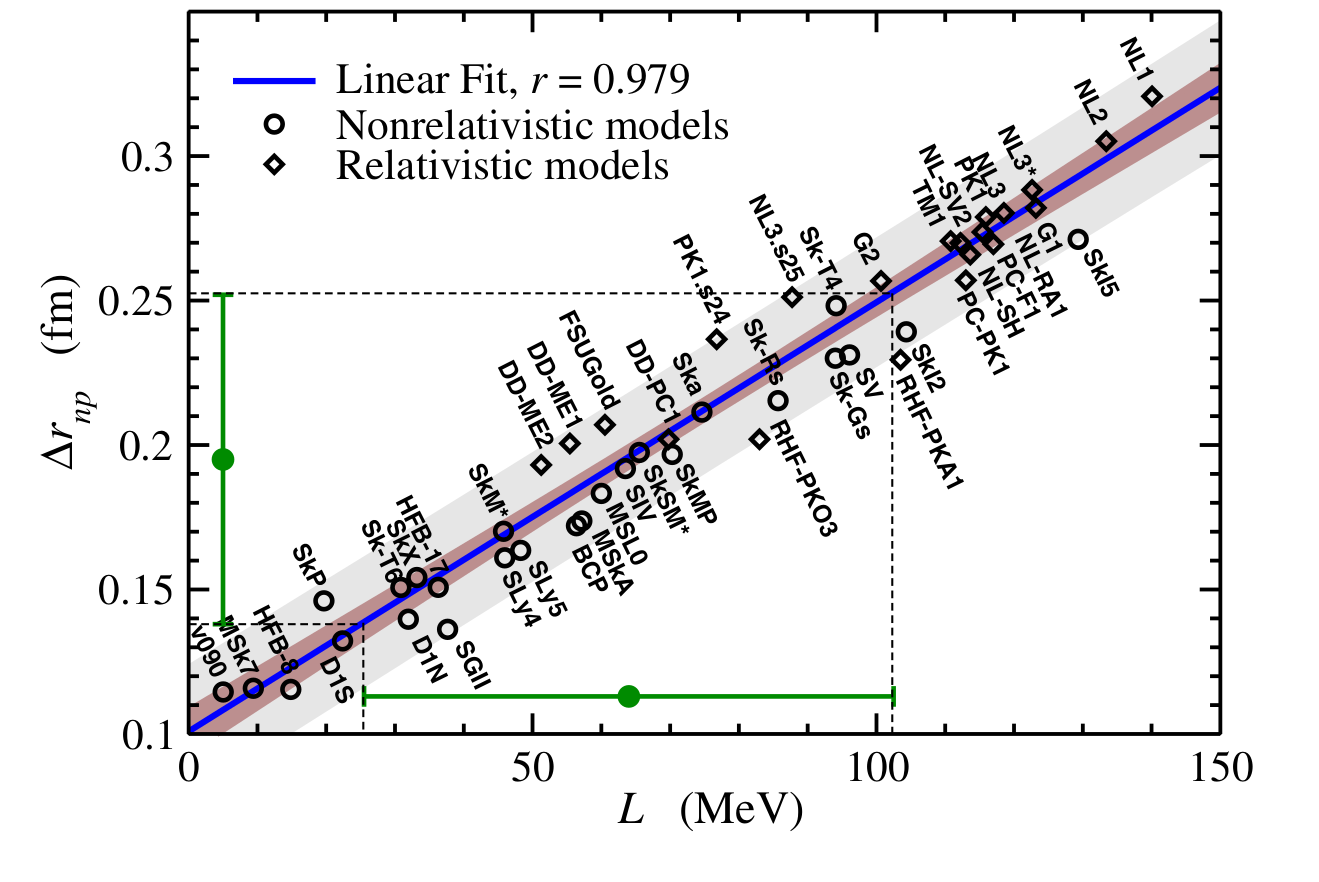
\includegraphics[width=0.5\linewidth]{R_skin_vs_L}
    \caption{Correlation between the neutron skin thickness of \Pb and the 
    slope of the symmetry energy ($L$). The linear fit is $\Delta r_{np} = 0.101 + 0.00147 L$.
    \cite{PhysRevLett.106.252501}}
\end{figure}

Being such an important parameter, great efforts have been devoted to extracting $S$ 
and $L$. By comparing Eq.~\ref{eq:modified-mass-formula-2} and \ref{eq:symmetry-energy},
we can directly obtain:
\begin{equation}
    S(\rho) \approx -a_A
% S(\rho) = -a_A + \frac{L}{3}\frac{\rho - \rho_0}{\rho_0}
\end{equation}
The problem is that this only tells the symmetry energy at the nuclear density ($\sim 1 \times 10^{44}\ \mathrm{m}^{-3}$).
It does not provide any information about the symmetry energy at other density values, 
particularly at the nuclear saturation density of approximately $1.5 \times 10^{44}\ \mathrm{m}^{-3}$, 
let along the density dependence of the symmetry energy. 

A more practical strategy to calculate $S(\rho)$ is the energy density functionals (EDF), 
which fits the binding energy throughout the nuclear mass table to find out the best EDF,
then use it to calculate $S(\rho)$. Fitting parameterizations are constrained
by nuclear densities, proton RMS radii and nuclear binding energies. 
The issue is many EDFs can fit equally well with these constraints, but have quite 
different $L$ values, as shown in Fig.~\ref{fig:neutron_EOS}.
An experiment that could identify $S$ ($L$) value without model dependence, 
would be helpful in understanding the symmetry energy and the EOS.
\begin{figure}[!h]
    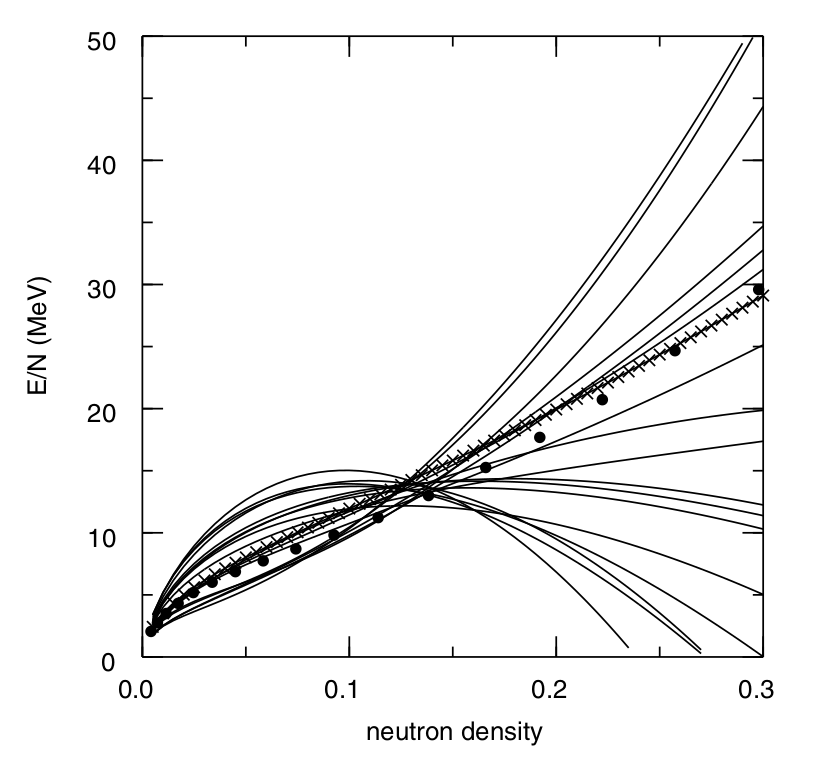
\includegraphics[width=0.48\linewidth]{S_vs_rho_n}
    \hfill
    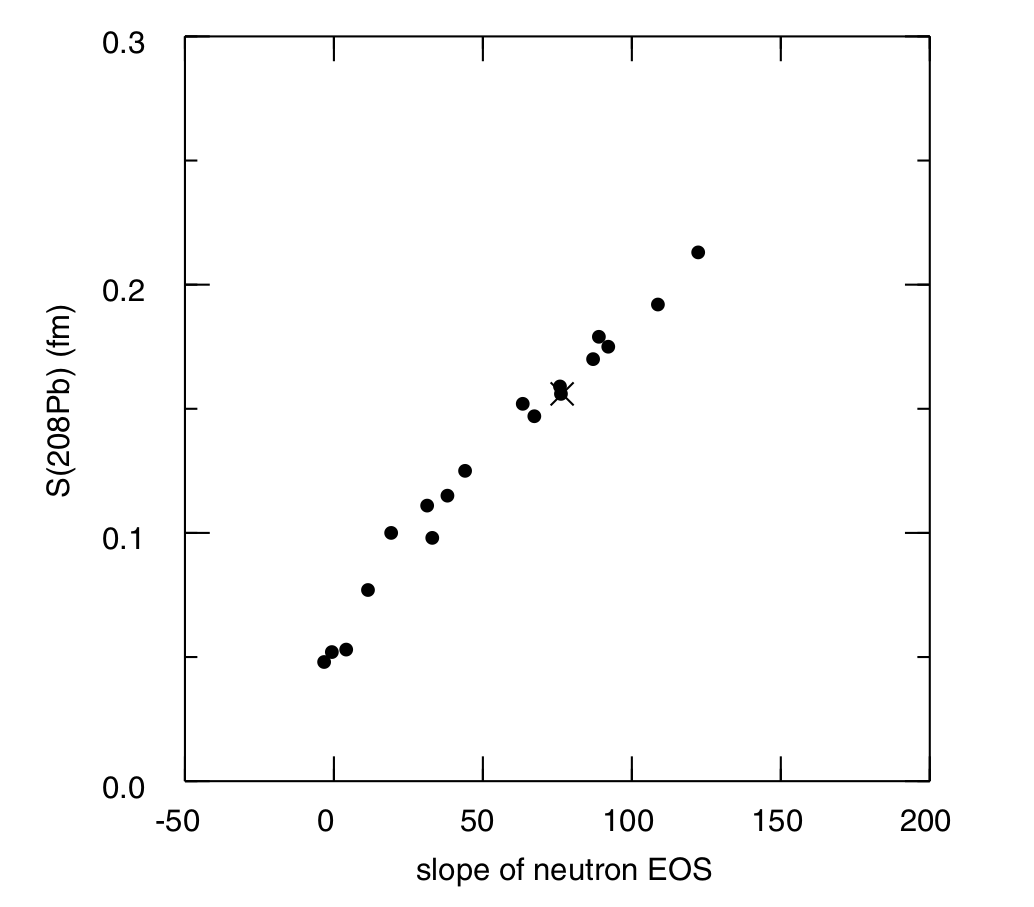
\includegraphics[width=0.49\linewidth]{S_Pb_in_S_N_EOS}
    \caption[Neutron EOS with different slope values]
    {Left: Neutron EOS for 18 Skyrme \cite{Skyrme} parameter sets. The filled circles represent
    the Friedman-Panharipande (FG) variational calculations and the crosses are SkX predictions
    \cite{PhysRevC.58.220}.
    It is apparent that different models exhibit significant variations in their symmetry energies.
    Right: Density dependence of the symmetry energy (in units of MeV $\mathrm{fm}^3$/neutron) 
    at $\rho_n = 0.1$~neutron/fm${}^3$ vs the neutron skin thickness in \Pb 
    for the 18 Skyrme parameter sets. The cross corresponds to SkX. 
    Determination of the neutron skin thickness in \Pb will greatly narrow down
    the list of possible candidates.
    \cite{PRL.85.5296}.
    }
    \label{fig:neutron_EOS}
\end{figure}
% experiments that measure L

% neutron skin
% The method to measure L in lab is to measure the neutron skin thickness of 
% neutron rich nuclei. For symmetric nuclei (N = Z), the protons and neutrons are
% expected to distribute uniformly. While for neutron-rich nuclei, the extra 
% neutrons are pushed out against the surface tension\cite{PRL.85.5296}, therefore
% forming a neutron skin. 
  
%%%%%%%%%%%%%%%%%%%%%%%%%%%%%%%%%%%%%%%%%%%%%%%%
\section{Nuclear Structure and Neutron Stars}
Unlike particle physics, which has a standard model to describe the fundamental particles and their interactions, there is no such standard model in nuclear physics that can accurately capture the static properties and dynamics of atomic nuclei, such as the ground state binding energy, nuclear size, and excitation spectrum.

The fundamental building blocks of nuclei are quarks and gluons. Theoretically, 
all properties of a nucleus can be derived directly from the interactions
of these elementary particles using QCD. Many groups work in this direction, 
attempting to derive nuclear structure from underlying QCD. 
Unfortunately, at the low energy scale where nuclei exist, the non-perturbative nature of 
QCD makes the problem so complicated that even the state-of-the-art lattice QCD
technique can only resolve a small nuclear system with a few nucleons.
This suggests that quarks and gluons are not the most suitable degrees of freedom to describe nuclei
using current techniques.

% first problem: nuclear forces governed by QCD, which is non-perturbative at low energy
Instead of quarks and gluons, nucleons and their intermediary particles, pions,
are a more natural choice of degrees of freedom for the description of nuclei
since they are the direct components of nuclei, 
This was the approach physicists used to study nuclear systems in the beginning (1930s \cite{10.1143/PTPS.1.1}). 
Many nuclear models were developed based on the meson-exchange phenomenology, called	% FIXME reference
phenomenological interactions, up until the mid-1990s.
With the uncovering of QCD, this approach was re-discovered from the aspect of QCD:
quarks and gluons are confined in colorless nucleons and pions, the nuclear force
is just the residual interaction between quarks and gluons. Since int is rooted 
in underlying QCD, it is appropriate to describe nuclear systems in terms of nucleons and pions.

%%%%%%%%%%%%%%%%%%%%%%%%
\subsection{Ab-initio Method}
Although it is still unknown how the nuclear force emerges from the underlying QCD interaction,
it is expected that both the force and the interaction should share the same properties, 
particularly the same symmetries and symmetry-breaking patterns. 
Among these properties, the spontaneously broken chiral symmetry is considered 
the most significant. With this in mind, S. Weinberg proposed a new framework
in the 1990s called chiral effective field theory ($\chi$EFT), which is an effective realization of the 
underlying QCD Lagrangian based on chiral symmetry \cite{WEINBERG1979327}.

% All possible terms that are consistent with the underlying QCD symmetry.

Ab-initio methods try to calculate the wave function of nuclei by solving the
many-body Schr\"{o}dinger equation:
\begin{equation}
    H\ket{\psi} = E\ket{\psi}
\end{equation}
where the Hamiltonian is
\begin{equation}
    H = T + V = \frac{1}{A} \sum_{i<j}^A \frac{(\vec{p}_i - \vec{p}_j)^2}{2m} 
	+ \sum_{i<j}^A V_{ij}^{NN} + \sum_{i<j<k}^A V_{ijk}^{NNN} + \cdots
\end{equation}

In $\chi$EFT, the potential must adhere to the same symmetries as QCD,
such as spacetime translation, rotation, parity transformation, and others. 
Most importantly, the potential should preserve the spontaneously broken chiral symmetry. 
Constrained by these symmetries, the operator for the potential takes the form of:
\begin{equation}
    \mathds{O}_V = \{\mathds{1}, \vec{\sigma}_i \cdot \vec{\sigma}_j, \vec{L} \cdot \vec{S}, S_{ij}\} 
	\times \{\mathds{1}, \vec{\tau}_i \cdot \vec{\tau}_j\}
\end{equation}
where $\vec{\sigma}_i \cdot \vec{\sigma}_j$ ($\vec{\tau}_i \cdot \vec{\tau}_j$) 
denotes the spin (isospin) interaction, 
$\vec{L} \cdot \vec{S}$ indicates the spin-orbit interaction and the tensor interaction
is represented by
\begin{equation}
    S_{ij}(\vec{x}) = 3(\vec{\sigma_i} \cdot \hat{\vec{x}})(\vec{\sigma}_j \cdot \hat{\vec{x}}) - \vec{\sigma}_i \cdot \vec{\sigma}_j
\end{equation}
where $\hat{\vec{x}}$ is the unit vector along vector $\vec{x}$.

The typical momentum (soft scale) in nuclei is of the order of $p \sim m_\pi \sim \mathds{O}(100\ \mathrm{MeV})$, 
while the short-range structure involving heavier meson (hard scale) is about 
$\Lambda_\chi \sim m_\rho \sim \mathds{O}(700 \ \mathrm{MeV})$. 
The clear gap between the soft and hard scales allows for the separation of the 
long-range force from the short-range one, as shown in Fig.~\ref{fig:nuclear_potential}. 
The term `effective' in the name of $\chi$EFT refers to the fact that only the 
long-range pion exchange in the low-energy scale will be considered, 
while heavier mesons will be integrated out as low-energy constants (LECs), 
which are phenomenologically fitted. 
\begin{figure}[!h]
    \centering
    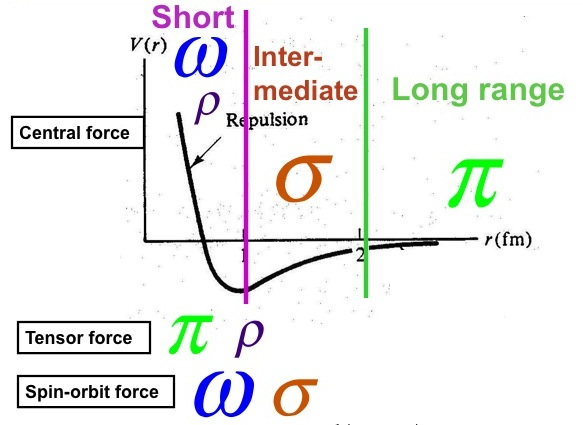
\includegraphics[width=0.5\linewidth]{nuclear_force}
    \caption{Separation of nuclear forces.}
    \label{fig:nuclear_potential}
\end{figure}

By employing the effective theory, one can expand the potential in terms of
$\left(\frac{Q}{\Lambda_\chi}\right)^\nu$, where Q is the momentum transfer
between two nucleons and $\Lambda_\chi$ is the cut-off scale where short-range 
interactions become important, and $\nu$ is the power that defines the order of
the interaction. The order of the expansion determines the accuracy of the calculation, 
with higher orders resulting in more accurate results, as illustrated in Fig.~\ref{fig:nuclear_interactions_in_order}.
\begin{equation}
    V = \sum_i V^{(i)} = V^{(0)}_{LO} + V^{(2)}_{NLO} + V^{(3)}_{NNLO} + V^{(4)}_{NNNLO} \cdots
\end{equation}
In this way, one can calculate nuclear force to any precision, by including
more higher order terms, if not limited by computing power.

\begin{figure}[!h]
    \centering
    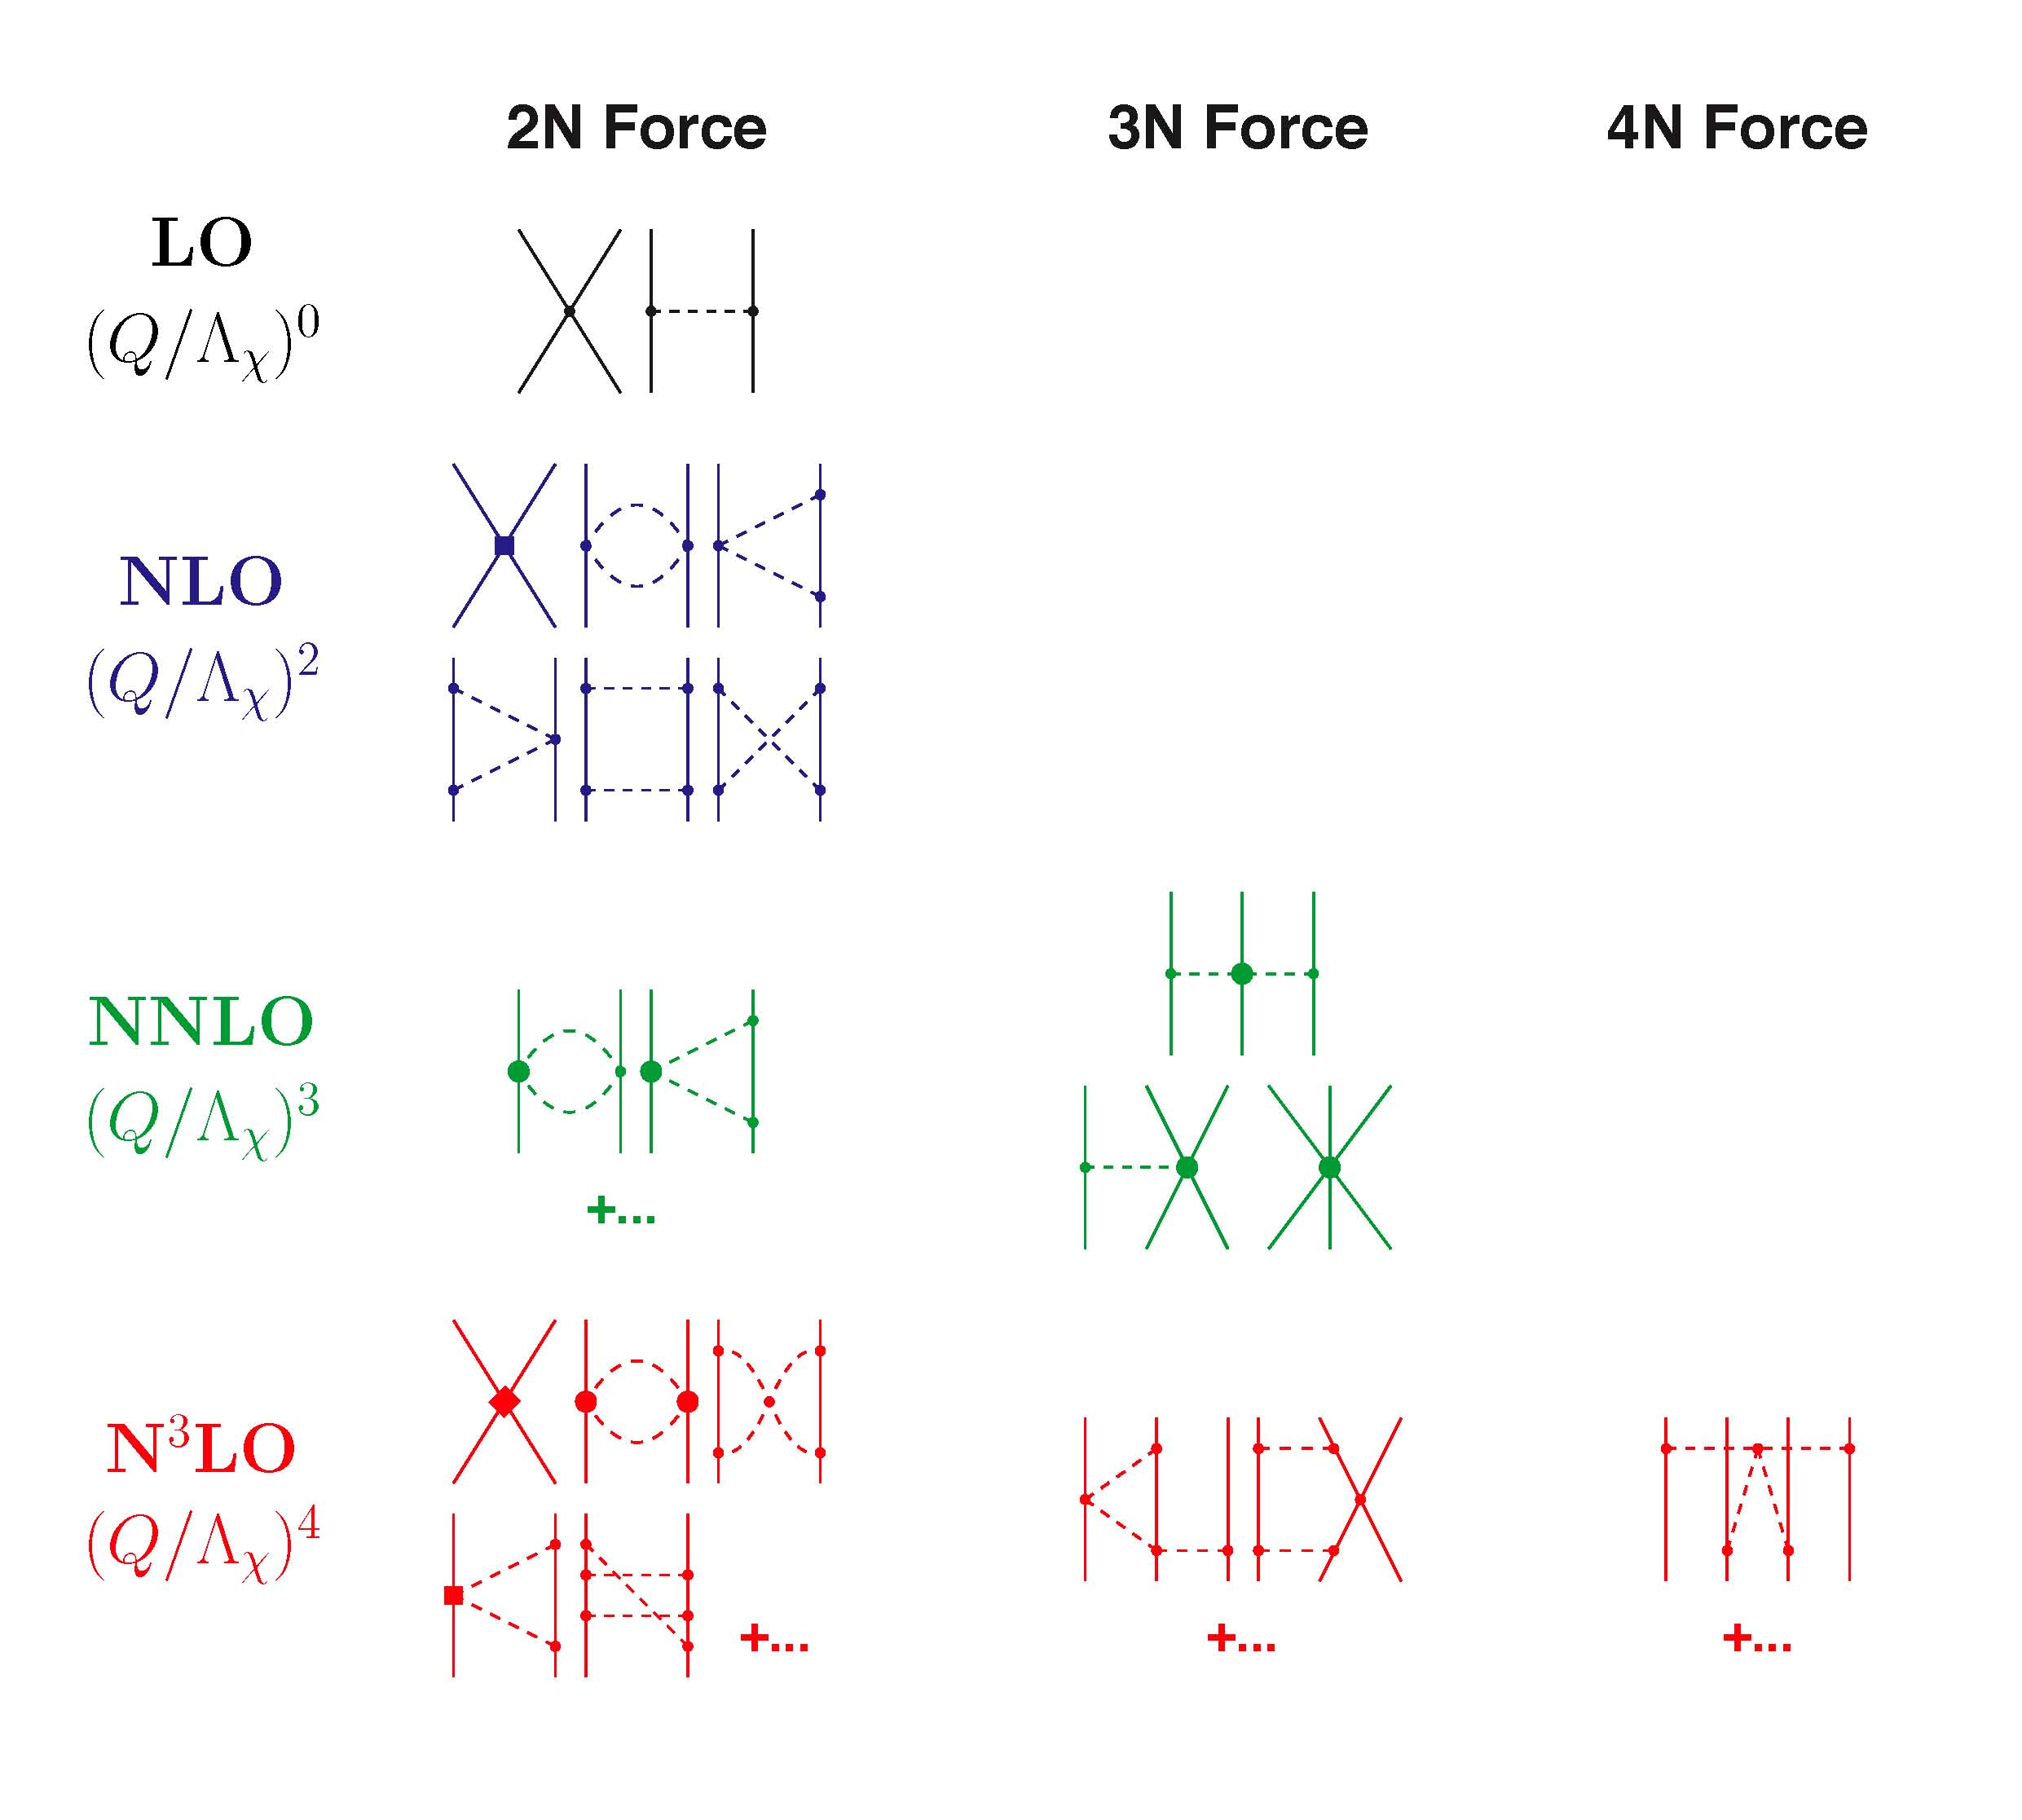
\includegraphics[width=0.5\linewidth]{nuclear_force_diagrams}
    \caption[Feynman diagrams for nuclear interactions]
    {Feynman diagrams for nuclear interactions. Solid lines refer to    
    nucleons while dashed lines represent exchanged pions. The first column     
    shows nucleon-nucleon force, and the following two columns correspond to the three-nucleon
    and four-nucleon forces. Rows show diagrams of leading order (LO), next-to-leading order (NLO) and so forth.}
    \label{fig:nuclear_interactions_in_order}
\end{figure}

For example, the $1\pi$-exchange potential between two nucleons is:
\begin{equation}
    V_{2N}^{1\pi} = -\frac{g_A^2}{4F_\pi^2}
    \frac{(\vec{\sigma}_1\cdot\vec{q})(\vec{\sigma}_2\cdot\vec{q})}{\vec{q}^2 + M^2_\pi}
    \vec{\tau}_1\cdot\vec{\tau}_2 
\end{equation}
where $g_A$ and $F_\pi$ are the axial-vector coupling constant and the pion 
decay constant.

After choosing the nuclear force potential, one can solve the Schr\"{o}dinger 
equation to obtain the eigenstate wave functions, which can then be used to
extract various properties. Ab-initio methods can be extended to nuclei with multiple nucleons using many-body techniques such as self-consistent Green's function, coupled cluster, and renormalization group.
% FIXME reference from each method

\begin{figure}[!h]
    \centering
    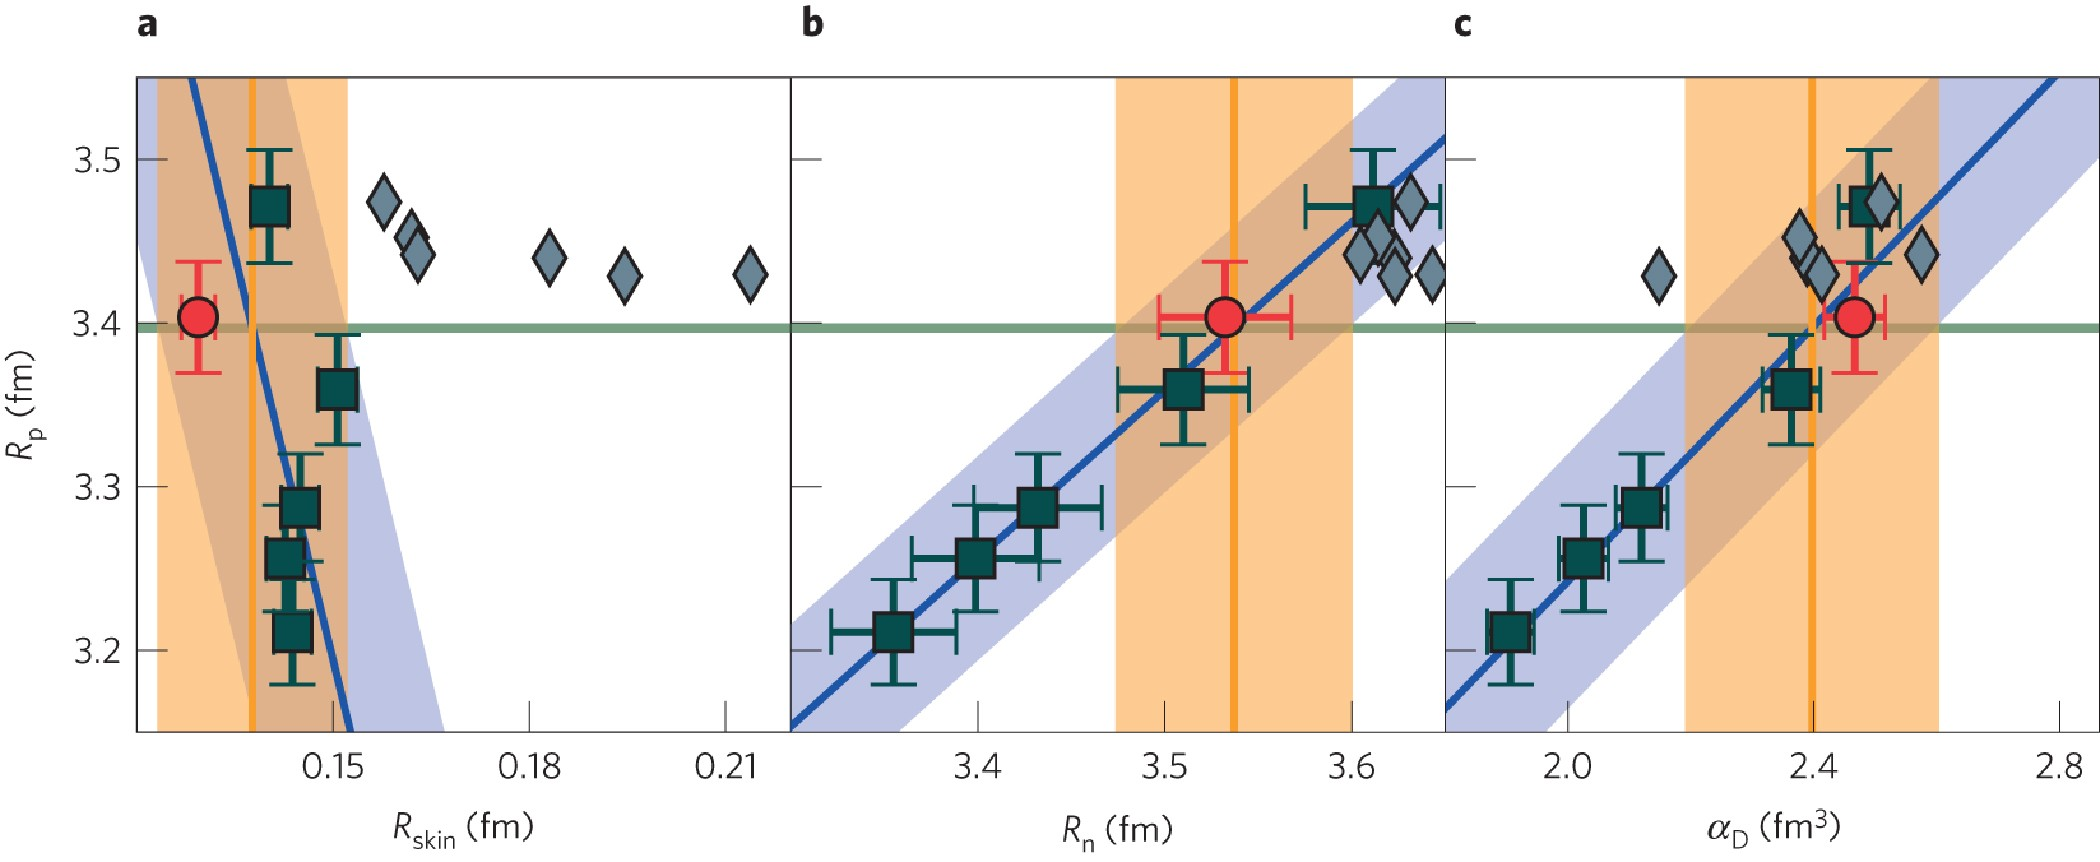
\includegraphics[width=0.8\linewidth]{ab_initio-Ca48_1}
    \caption[An ab-initio calculation of the neutron skin thickness of \Ca.]
    {An ab-initio calculation of the neutron skin thickness of \Ca.
    From left to right, the neutron skin thickness (a), neutron radius (b) and
    electric dipole polarizability (c) of \Ca are plotted against its proton 
    radius. The ab-initio predictions are shown as red circles and dark squares,
    while DFT results are represented by gray diamonds. The blue line represents 
    a linear fit to ab-initio predictions and the blue band represents the corresponding
    uncertainty of the blue line. The experimental value of $R_p$ is marked by 
    the horizontal green line, ant its intersection with the blue line and blue band yields
    the vertical orange line and orange band, respectively. \cite{Hagen2016}.}
\end{figure}

\begin{comment}
Deviation of ab-initio result and observation for heavy nuclei indicates the 
importance of higher-order interactions.

\begin{equation}
    \CL_{eff} = \CL_{\pi\pi} + \CL_{\pi N} + \CL_{NN} + \cdots
\end{equation}

three-nucleon forces are hard to observe directly, they increase the pressure of
neutron matter and therefore the neutron skin thickness of both \Pb and \Ca.

three-nucleon force term
\begin{itemize}
    \item Long-range two-pion exchange
    \item Medium-range one-pion exchange
    \item Short range three-nucleon contact
\end{itemize}
\end{comment}
%%%%%%%%%%%%%%%%%%%%%%%%
\subsection{Nuclear Density Functional Theory (DFT)}
% The second problem is many-body problem
While ab-initio methods have been successful in calculating properties of light 
and some medium nuclei, they currently lack the computational resources needed to
handle heavy nuclei, due to the exponential growth in the number of nucleons.
As an alternative approach, nuclear DFT begins with nuclear phenomenology and 
attempts to derive the underlying QCD theory from there.

The DFT method originates from solid-state physics, where it was first used to 
tackle the many-electron problem. It is based on the Hohenberg and Kohn (HK) theorem \cite{PhysRevC.57.3430}, 
which states that the total energy of a system can be expressed in terms of its
fermion (electron) density (density functional).
Minimizing this density functional leads to the ground-state density distribution, 
thereby reducing the number of degrees of freedom from 3N to 3. The only problem 
is that the HK theorem does not provide a prescription for constructing the density functional.

Unlike the Coulomb interaction, nuclear interactions are more complex because 
the three-nucleon interaction cannot be ignored. Fortunately, nuclear interactions
are short-range, and experimental observations suggest that nucleons in nuclei
do not interact frequently because their mean free path is about or larger than 
the nuclear radius. This validates the use of the mean-field method, where nucleons
move in a one-body potential that averages over interactions with all other nucleons. 
The Woods-Saxon potential is the most commonly used potential for this purpose.

Given the Hamiltonian of a nuclear system:
\begin{equation}
    H = \sum_i^N -\frac{\hbar^2}{2m}\nabla_i^2 + \frac{1}{2} \sum_{i\neq j=1}^N V(i, j)
\end{equation}
The Hartree-Fock (HF) energy of the system is:
\begin{equation}
    E_{HF}(\rho) = \bra{\Phi} H \ket{\Phi}
\end{equation}
where $\ket{\Phi}$ is the Slater determinant made up with the single-particle wave 
function $\ket{\phi}$.

The HK theorem states that:
\begin{equation}
    \frac{\delta}{\delta\rho(\vec{r})} \left( E_{HF} - \epsilon\int d^3r' \phi^*_j(\vec{r}')\phi_j(\vec{r}') \right) = 0
\end{equation}
With
\begin{equation}
    \rho(\vec{r}) = \sum_i^N \phi_i^*(\vec{r})\phi_i(\vec{r})
\end{equation}
It leads to the well-known HF equations:
\begin{equation}
    \begin{aligned}
	-\frac{\hbar^2}{2m}\nabla^2\phi_j(\vec{r}) 
	+ \sum_{l=1}^N \int d^3\vec{r}' \phi^*_l(\vec{r}') V(\vec{r}, \vec{r}') (\phi_l(\vec{r}')\phi_j(\vec{r}) - \phi_l(\vec{r}')\phi_l(\vec{r}'))
	&= \epsilon_j\phi_j(\vec{r})	\\
	\bra{j}\frac{-\hbar^2}{2m}\nabla^2\ket{j} + \sum_{l=1}^N \bra{jl}V(1-P_{12})\ket{jl} = \epsilon_j
    \end{aligned}
\end{equation}
where $P_{12}$ exchanges particles 1 and 2. So the total energy is:
\begin{equation}
    E_{HF} = T + \frac{1}{2}\sum_{jl} \int d^3r d^3r' \phi_j^*(\vec{r}')\phi_l^*(\vec{r}')V(\vec{r}, \vec{r}') (\phi_j(\vec{r}')\phi_l(\vec{r}') - \phi_l(\vec{r}')\phi_j(\vec{r}'))
\end{equation}
where T is the kinetic energy.

Given the interaction (the potential term $V(\vec{r}, \vec{r}')$), 
one can calculate the density distribution, and consequently, the total 
energy of the system as well as other relevant properties. One widely used model
in this paradigm is the Skyrme force.
\begin{equation}
    \begin{aligned}
	V_{\text{Skyrme}}(\vec{r}_1, \vec{r}_2) &= t_0 (1 + x_0 P_\sigma)\delta(\vec{r}_1 - \vec{r}_2) 
	+ \frac{1}{2}t_1 (1 + x_1 P_\sigma) \left( \vec{k}^{\dag2}\delta(\vec{r}_1 - \vec{r}_2) + \delta(\vec{r}_1 - \vec{r}_2)\vec{k}^2 \right)    \\
	&+ t_2(1 + x_2 P_\sigma)\vec{k}^\dag \cdot \delta(\vec{r}_1 
	    - \vec{r}_2)\vec{k} + \frac{1}{6} t_3 (1 + x_3 P_\sigma)\delta(\vec{r}_1 - \vec{r}_2) \rho^\alpha\left( \frac{\vec{r}_1 + \vec{r}_2}{2} \right) \\
	&+ iW_0 (\vec{\sigma}_1 + \vec{\sigma}_2) \cdot \vec{k}^\dag \times \delta(\vec{r}_1 - \vec{r}_2) \vec{k}
    \end{aligned}
\end{equation}
which has up to 10 parameters that are constrained by experimental data, such as
nuclear mass, radius and binding energy.

\bigskip
By measuring the neutron skin thicknesses of \Pb and \Ca, we can verify the
credibility of these ab-initio and DFT methods, and greatly constraint the
parameter space of each model. This can helps in developing a more general nuclear theory.

%%%%%%%%%%%%%%%%%%%%%%%%%%%%%%%%%%%%%%%%%%%%%%%%
\subsection{Neutron Stars}
% Take the neutron star \cite{Lattimer.2001} as an example. 
A neutron star is the densest celestial body known, the pressure due to gravity is so strong
that even atoms inside the star collapse, crushing together electrons
and protons into neutrons, giving the star its name. Neutron stars are primarily
observed as pulsars or in binary systems. Exploring the basic properties of
neutron stars can shed light on fundamental questions shared between nuclear physics 
and astrophysics. For example:
\begin{itemize}
    \item What is the high density phase of QCD?
    \item What is the structure of many compact and energetic celestial bodies?
	and what determines their EM, neutrino and gravitational radiations?
\end{itemize}

Despite a 18 orders of magnitude difference in size (fm vs km), 
the neutron star and the nuclear neutron skin share the same EOS. 
It is the pressure of neutron-rich matter that supports the neutron skin 
against its surface tension and a neutron star against its own gravity. 
Thus, the neutron skin thickness and the size of a neutron star are connected
through the pressure of neutron-rich matter, specifically the density dependence 
of the symmetry energy $L$.
The larger the neutron skin thickness, the larger the symmetry energy slope $L$,
the larger the pressure, and therefore the larger the radius of a neutron star, 
at the same mass. 

Quantitatively, a neutron star is predominantly composed of neutrons, with only 
a few protons, resulting in a high isospin asymmetry parameter, $\beta \approx 1$. 
Thus, Eq.~\ref{eq:symmetry-energy} can be simplified to:
\begin{equation}
    e(\rho) = e(\rho, 0) + S(\rho)
\end{equation}
Pressure is derived to be:
\begin{equation}
    P = \rho^2\frac{de}{d\rho} \simeq \rho^2 \frac{dS}{d\rho} \approx \frac{L\rho^2}{3\rho_0}  \\
\end{equation}
It is seen that the pressure of neutron-rich matter depends on $L$. 

For a cold neutron star, the correlation between its radius and pressure is \cite{Lattimer.2001}:
\begin{equation}
    R \simeq C(\rho, M) P^{0.23-0.26} 
\end{equation}
where $C$ is a coefficient that depends on the density $\rho$ and the stellar mass M,
and P is evaluated at the density $\rho$. This formula works for $\rho$ in the 
range of 1 to 1.5 times the nuclear saturation density.

Once the value of $L$ is fixed by an experimental measurement of the neutron skin 
thickness in \Pb, one is able to calculate the radius of a cold neutron star,
providing guidance for experimental observations.
% A neutron star is expected to have a solid crust over a liquid core. The phase transition
% from the high density core to the low density crust depends on the properties of the
% neutron-rich matter. Specifically, the density dependence of the symmetry energy $L$.
% A thicker neutron skin in \Pb indicates a large value of $L$, or rapid rise of
% the symmetry energy with density, which leads to a low transition density in a neutron
% star.



\begin{comment}
%%%%%%%%%%%%%%%%%%%%%%%%%%%%%%%%%%%%%%%%%%%%%%%%%%%%%%%%%%%%%%%%%%%%%%%%
\section{Physics Beyond the Standard Model (SM)} 
% leptoquark, Z', SUSY
PVES experiments are always a promising avenue for the search of physics beyond the SM in precision frontier,
because of the high precision they can achieve.
The Feynman diagrams from flavor-conserving PVES are shown in Fig.~\ref{fig:BSM}
\begin{figure}[!h]
    \centering
\feynmandiagram[small, vertical' = a to b]{
    i1 [particle = $e^-$] -- [fermion] a -- [fermion] o1 [particle = $e^-$],
    a -- [photon, edge label={Q}, edge label'=$\gamma$] b,
    i2 [particle = N] -- [fermion] b -- [fermion] o2 [particle = N],
    };
\feynmandiagram[small, vertical' = a to b]{
    i1 [particle = $e^-$] -- [fermion] a -- [fermion] o1 [particle = $e^-$],
    a -- [scalar, edge label={Q}, edge label'=Z] b,
    i2 [particle = N] -- [fermion] b -- [fermion] o2 [particle = N],
    };
\feynmandiagram[small, vertical' = a to b]{
    i1 [particle = $e^-$] -- [fermion] a -- [fermion] o1 [particle = $e^-$],
    a -- [scalar, edge label={Q}, edge label'=Z'] b,
    i2 [particle = N] -- [fermion] b -- [fermion] o2 [particle = N],
    };
    \caption{Feynman diagrams of elastic eA scattering.}
    \label{fig:BSM}
\end{figure}

Knowing that the EM interaction is much larger than the neutral weak current and
the possible new interaction, we can approximate:
\begin{equation}
    |\CA_\gamma + \CA_Z + \CA_{\text{new}}|^2 \approx A^2_\gamma\left[ 1 + 2\frac{\CA_Z}{\CA_\gamma}
    + 2\frac{\CA_{\text{new}}}{\CA_\gamma} \right]
\end{equation}
If the new interaction amplitude $\CA_{\text{new}}$ is comparable to $\CA_Z$ or our measurement 
of $\CA_Z$ is precise enough, we will be able to distinguish any possible deviation,
prompting on the existence of new physics.

Any PV interaction can be described in the SM as:
\begin{equation}
    \mathcal{L}_{PV}  = -\frac{G_F}{\sqrt{2}}\left[ 
	\bar{e}\gamma_\mu\gamma_5 e (C_{1u}\bar{u}\gamma^\mu u + C_{1d}\bar{d}\gamma^\mu d)
      + \bar{e}\gamma_\mu e (C_{2u}\bar{u}\gamma^\mu\gamma^5 u + C_{2d}\bar{d}\gamma^\mu \gamma^5d)
	\right]
% https://doi.org/10.1140/epja/i2006-09-011-8
\end{equation}
where $C_{iq}$ is the constant coefficient predicted by the SM:
\begin{equation}
    \begin{gathered}
	C_{1q} \equiv 2g_A^e g_V^q	\qquad C_{2q} \equiv 2g_V^e g_A^q   \\
	g_A = I_3   \qquad g_V = I_3 - 2Q\sin^2\theta_W
    \end{gathered}
\end{equation}
These coefficients or their combinations give favorable experimental observables:
\begin{equation}
    \begin{aligned}
	C_{1u} &= -\frac{1}{2} + \frac{4}{3}\sin^2\theta_W   \\
	C_{1d} &= \frac{1}{2} - \frac{2}{3}\sin^2\theta_W   \\
	C_{2u} &= -\frac{1}{2} + 2\sin^2\theta_W   \\
	C_{2d} &= \frac{1}{2} - 2\sin^2\theta_W   \\
    \end{aligned}
    \Longrightarrow
    \begin{aligned}
	\tilde{\alpha} &= -C_{1u} + C_{1d} = -(1-2\sin^2\theta_W)	\\
	\tilde{\beta} &= -C_{2u} + C_{2d} = -(1-4\sin^2\theta_W)	\\
	\tilde{\gamma} &= -C_{1u} - C_{1d} = \frac{2}{3}\sin^2\theta_W	\\
	\tilde{\delta} &= -C_{2u} - C_{2d} = 0	\\
    \end{aligned}
\end{equation}
where $\theta_W$ is the weak mixing angle.

Most PVES experiments measure the weak charge (the weak mixing angle) directly, like
E158 at SLAC and the upcoming MOLLER at JLab. Compared to these experiments, PREX/CREX
are less sensitive to new physics, because PREX/CREX measurements involve many 
weak charge sources inside a nucleus and their distribution. Though new physics
is not the main goal of the PREX/CREX collaboration, the possibility for new physics 
is not completely cut off.
\end{comment}

%%%%%%%%%%%%%%%%%%%%%%%%%%%%%%%%%%%%%%%%%%%%%%%%
\section{Symmetry and Asymmetry}
Symmetry is a powerful framework in modern physics. For any physical system, 
by applying proper symmetry requirements, one can derive or predict
the Lagrangian of the system, which in turn yields its properties and Equation of Motion (EOM).

Common space-time symmetries can be categorized into continuous and discrete symmetries. 
Continuous symmetries include translation, rotation and boost, 
while discrete symmetries involve space reflection (P) and time reversal (T).
Another important discrete symmetry is charge conjugation (C).

Giving their curcial role, the violation of symmetries holds significant importance.
Presently, it is widely accepted that continuous symmetries are conserved 
by all interactions, while weak interaction violates certain discrete symmetries, 
specifically C, P, and their combination CP. There are some speculations that 
the strong interaction can violate the CP symmetry, but no
experimental observation reported thus far \cite{MANNEL2007170}.

%%%%%%%%%%%%%%%%%%%%%%%%%%%%%%%%%%%%%%%%%%%%%%%%
\subsection{Parity Symmetry}
Parity symmetry is a discrete symmetry that asserts the equivalence of physical 
laws between the mirror (reflection) world and the real world, as shown in 
Fig.~\ref{fig:space_reflection}. 
\begin{figure}[!h]
    \centering
    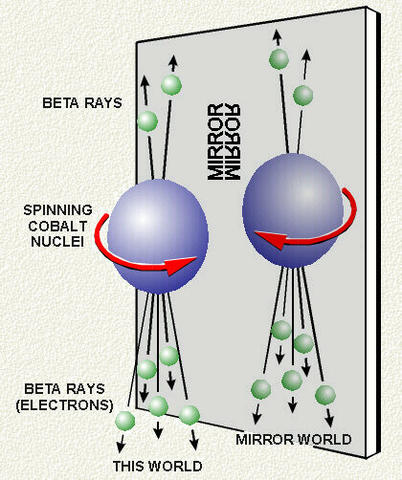
\includegraphics[width=0.4\linewidth]{parity}
    \label{fig:space_reflection}
    \caption{Schematic plot of space reflection.}
\end{figure}

The parity operation will flip the sign of any spatial coordinate:
\begin{equation}
    P: \vec{r} \rightarrow -\vec{r}
\end{equation}
The same for any spatial vector, like momentum ($\vec{p}$), angular momentum ($\vec{L}$)
and the EM vector potential ($\vec{A}$).

In the language of QM, the parity operator ($\hat{\pi}'$) will transform 
a wave function, as shown in Eq.~\ref{eq:parity_transformation}.
\begin{equation}
    \hat{\pi}'\psi(x, y, z) = \eta \psi(-x, -y, -z)
    \label{eq:parity_transformation}
\end{equation}
where $\eta$ is a coefficient picked up by the transformation. It is expected that
the state goes back to itself after 2 times of parity transformations:
\begin{equation}
    |\hat{\pi}'^2 \psi(x, y, z)|^2 = |\psi(x, y, z)|^2
    \qquad
    \hat{\pi}'\psi(x, y, z) = e^{i\phi/2}\psi(-x, -y, -z)
\end{equation}
which means $\hat{\pi}'$ is a unitary operator. The pick up phase can
be absorbed into the operator to get the new parity operator (what we use hereafter): 
\begin{equation}
    \hat{\pi} = \hat{\pi}'e^{-i\phi/2}
\end{equation}
Then we have
\begin{equation}
    \hat{\pi}^2 = 1 
\end{equation}
So $\hat{\pi}$ has eigenvalues of $p = \pm 1$. States with eigenvalue of +1 are called
parity-even states and the others with eigenvalue of -1 the parity-odd states.

For a scalar potential, $V(\vec{r}) = V(r)$ ($[\hat{\pi}, V] = 0$), the parity 
operator $\hat{\pi}$ commutes with the Hamiltonian ($[\hat{\pi}, \CH] = 0$). 
Therefore, the energy eigenstates are also eigenstates of $\hat{\pi}$. 
Among these states, the orbital angular momentum eigenstates are
particularly interesting. Given an orbital angular momentum $\vec{L}$ with z-axis projection
$L_z$, one will have:
\begin{equation}
    \hat{\pi}\ket{\vec{L}, L_z} = (-1)^L\ket{\vec{L}, L_z}
\end{equation}

Another quantity similar to orbital angular momentum in many aspects but
distinct in terms of parity is spin. Spin, like orbital angular momentum, 
is an angular momentum, but it is an intrinsic property rather than a result
of space-time motion. Unlike $\hat{\pi}$, which is an operation of space, 
spin is not affected by $\hat{\pi}$. Consequently, the parity of a spin state
is arbitrary assigned as long as particles and their antiparticles have opposite
parities. For instance, electrons, protons and neutrons are assigned even parity 
while their antiparticles have odd parity.

Now, let us delve into the concept of helicity, which represents the projection of the 
spin onto the direction of momentum:
\begin{equation}
    H \equiv \frac{\vec{s}\cdot \vec{p}}{|\vec{s}\cdot\vec{p}|}
\end{equation}
If a particle's spin is aligned (opposite) to its momentum, we refer to it as a
right-handed (left-handed) particle. When we apply the parity operator to a helicity
eigenstate, the helicity gets reversed due to the flip in momentum's sign, while 
the spin remains unchanged. This can be observed in Fig.~\ref{fig:parity_eA_scattering_1}.
\begin{figure}[h!]
    \centering
    \begin{subfigure}[c]{0.44\linewidth}
	\begin{tikzpicture}[scale=0.8]
	    \begin{feynman}[transform shape]
		\vertex (i1) {$e^-$};
		\vertex [right=1.0cm of i1, inner sep=-2pt] (inspin) {\AxisRotator};
		\vertex [right=2.3cm of inspin] (ip);
		\vertex [right=2.8cm of ip] (i2) {A};
		\vertex [above right = 2cm and 2cm of ip] (o1) {$e^-$};
		\vertex [above right = 1cm and 1cm of ip] (outspin) {\AxisRotator[rotate=45]};
		\vertex [below left = 2cm and 2cm of ip] (o2) {A};

		\diagram* { {[edge=fermion]
		    (i1) --[edge label=$\vec{k}$] (ip) [dot] --[edge label = $\vec{k}'$] (o1),
		    (i2) --[edge label=$\vec{p}$](ip) [dot] -- [edge label = $\vec{p}'$]  (o2)},
		};
	    \end{feynman}
	\end{tikzpicture}
    \end{subfigure}
    $\overset{\hat{\pi}}{\Longrightarrow}$
    \hspace{0.2cm}
    \begin{subfigure}[c]{0.44\linewidth}
	\begin{tikzpicture}[scale=0.8]
	    \begin{feynman}[transform shape]
		\vertex (i1) {A};
		\vertex [right=2.8cm of i1] (ip);
		\vertex [right=2.3cm of ip, inner sep=-2pt] (inspin) {\AxisRotator};
		\vertex [right=1.0cm of inspin] (i2) {$e^-$};
		\vertex [above right = 2cm and 2cm of ip] (o1) {A};
		\vertex [below left = 1cm and 1cm of ip] (outspin) {\AxisRotator[rotate=45]};
		\vertex [below left = 2cm and 2cm of ip] (o2) {$e^-$};

		\diagram* { {[edge=fermion]
		    (i1) --[edge label=$\vec{p}$] (ip) [dot] --[edge label = $\vec{p}'$] (o1),
		    (i2) --[edge label=$\vec{k}$](ip) [dot] -- [edge label = $\vec{k}'$]  (o2)},
		};
	    \end{feynman}
	\end{tikzpicture}
    \end{subfigure}
    \caption{Parity transformation of the eA scattering}
    \label{fig:parity_eA_scattering_1}
\end{figure}

If parity is not conserved, a discrepancy will arise between the two scattering 
processes depicted in Fig.~\ref{fig:parity_eA_scattering_1}, which aligns with 
the measurement conducted in PREX-II/CREX. 
% This distinction is attributed to the presence of an interference term. 
In experimental practice, it is more convenient to reverse the spin direction rather than the momentum direction, as exemplified in Fig.~\ref{fig:parity_eA_scattering_2}, which serves as an equivalent representation of Fig.~\ref{fig:parity_eA_scattering_1}.
\begin{figure}[h!]
    \centering
    \begin{subfigure}[c]{0.48\linewidth}
	\begin{tikzpicture}[scale=0.8]
	    \begin{feynman}[transform shape]
		\vertex (i1) {$e^-$};
		\vertex [right=1.0cm of i1, inner sep=-2pt] (inspin) {\AxisRotator};
		\vertex [right=2.3cm of inspin] (ip);
		\vertex [right=2.8cm of ip] (i2) {A};
		\vertex [above right = 2cm and 2cm of ip] (o1) {$e^-$};
		\vertex [above right = 1cm and 1cm of ip] (outspin) {\AxisRotator[rotate=45]};
		\vertex [below left = 2cm and 2cm of ip] (o2) {A};

		\diagram* { {[edge=fermion]
		    (i1) --[edge label=$\vec{k}$] (ip) [dot] --[edge label = $\vec{k}'$] (o1),
		    (i2) --[edge label=$\vec{p}$](ip) [dot] -- [edge label = $\vec{p}'$]  (o2)},
		};
	    \end{feynman}
	\end{tikzpicture}
    \end{subfigure}
    \begin{subfigure}[c]{0.48\linewidth}
	\begin{tikzpicture}[scale=0.8]
	    \begin{feynman}[transform shape]
		\vertex (i1) {$e^-$};
		\vertex [right=1.0cm of i1, inner sep=-2pt] (inspin) {\AxisRotatorReversed};
		\vertex [right=2.3cm of inspin] (ip);
		\vertex [right=2.8cm of ip] (i2) {A};
		\vertex [above right = 2cm and 2cm of ip] (o1) {$e^-$};
		\vertex [above right = 1cm and 1cm of ip] (outspin) {\AxisRotatorReversed[rotate=45]};
		\vertex [below left = 2cm and 2cm of ip] (o2) {A};

		\diagram* { {[edge=fermion]
		    (i1) --[edge label=$\vec{k}$] (ip) [dot] --[edge label = $\vec{k}'$] (o1),
		    (i2) --[edge label=$\vec{p}$](ip) [dot] -- [edge label = $\vec{p}'$]  (o2)},
		};
	    \end{feynman}
	\end{tikzpicture}
    \end{subfigure}
    \caption{Equivalent plot of Fig.~\ref{fig:parity_eA_scattering_1}: flip spin 
    instead of momentum.}
    \label{fig:parity_eA_scattering_2}
\end{figure}
%%%%%%%%%%%%%%%%%%%%%%%%%%%%%%%%%%%%%%%%%%%%%%%%
\subsection{Parity Violation}
\begin{figure}[!h]
    \centering
    \begin{tikzpicture}[decoration={markings, 
	mark=at position 0.5 with {\arrow{stealth}}}
	]
	\begin{scope}
	    \coordinate (O) at (0, 0);
	    \filldraw[black] (O) circle (1pt);
	    \node[red, above] at (O) {$G_F$};
	    \draw[postaction={decorate}] (-2, 0) node[above] {n} -- +(2, 0);
	    \draw[postaction={decorate}] (O) -- +(2, 0)node[above] {$p$} ;
	    \draw[postaction={decorate}] (O) -- (35:2) node[above, sloped] {$e^-$};
	    \draw[postaction={decorate}] (O) -- (-35:2) node[above, sloped] {$\bar{\nu}_e$};
	\end{scope}

	\begin{scope}[xshift=5cm]
	    \coordinate (O) at (0, 0);
	    \filldraw[black] (O) circle (1pt);
	    \node[red, above] at (O) {$G_F$};
	    \draw[postaction={decorate}] (-2, 0) node[above] {n} -- +(2, 0);
	    \draw[postaction={decorate}] (O) -- +(2, 0)node[above] {$p$} ;
	    \draw[postaction={decorate}] (O) -- (35:2) node[above, sloped] {$e^-$};
	    \draw[postaction={decorate}] (-35:2) node[above, sloped] {$\nu_e$} -- (O);
	\end{scope}
    \end{tikzpicture}
    \caption{Fermi's interpretation of beta decay, current $j_{n \rightarrow p}$ 
    convert $n$ into $p$ and current $j_{\nu_e \rightarrow e}$ creates $(e, \ \bar{\nu}_e) $
    pair.}
\end{figure}
The history of parity violation can be traced back to the early days of particle physics. 
In 1933, Fermi proposed the concept of four-fermion interaction, also known as 
Fermi's interaction, to explain beta decay \cite{Fermi1934}. 
This interaction serves as a low-energy approximation of the weak interaction. 
In Fermi's theory, by drawing an analogy to the EM interaction where an electron
emits a photon: $\CM = ej_\mu^{em} A^\mu$, $\beta$ decay was interpreted 
as the emission of an electron and an electron antineutrino $(e, \bar{\nu}_e)$ pair. 
During the process, a neutron transforms into a proton, and thus, it involves 
the coupling of two currents:
\begin{equation}
    \CM = G_F (\bar{p} \mathds{O}^\mu n)(\bar{e} \mathds{O}_\mu \nu_e) 
	= G_F j^\mu_{(n\rightarrow p)} j_\mu^{(\nu_e\rightarrow e)}
\end{equation}
Where $G_F = 1.166 \times 10^{-5} \mathrm{GeV}^{-2}$ is the coupling constant that 
can be experimentally determined, and $\mathds{O}$ represents 
the possible operators. Among the five possible Lorentz invariant bilinear forms 
(Scalar (S: $\mathds{O} = \mathds{1}$), pseudo-scalar (P: $\mathds{O} = \gamma^5$), 
Vector (V: $\mathds{O} = \mathds{\gamma^\mu}$), Axial vector (A: $\mathds{O} = \gamma^\mu\gamma^5$) 
and Tensor (T: $\mathds{O}=\sigma^{\mu\nu} = \frac{i}{2}(\gamma^\mu\gamma^\nu - \gamma^\nu\gamma^\mu)$)),
Fermi selected the vector current to maintain consistency with the EM interaction:
$j^\mu = \bar{u} \gamma^\mu u$.

%%%%%%%%%%%%%%%%%%%%%%%%
\subsubsection{V-A Theory}
In 1956, T. D. Lee and C. N. Yang, both of whom were students of Fermi, put forward
the groundbreaking concept of parity violation to address the $\tau-\theta$ puzzle \cite{PhysRev.105.1671}, 
and they achieved success. Just one year later, their hypothesis was experimentally tested
by Wu et al. in the decay of polarized ${}^{60}$Co nuclei \cite{PhysRev.105.1413}, 
providing evidence that parity is not conserved in weak interactions and 
consequently, the weak current is not pure vector-like. 
The experimental observation of maximal violation of parity, where left-handed 
electrons interact weakly while right-handed electrons do not \cite{PhysRev.109.1015}, 
prompted Sudarshan and Marshak \cite{PhysRev.109.1860.2}, as well as 
Feynman and Gell-Mann \cite{PhysRev.109.193}, to revise Fermi's theory. 
They introduced a new current in place of the vector current to account for
parity violation:
\begin{equation}
    \CM = \frac{G_F}{\sqrt{2}}(\bar{p} \gamma^\mu(\mathds{1} - \gamma^5) n) (\bar{e} \gamma_\mu(\mathds{1} - \gamma^5) \nu_e)
\end{equation}
The factor of $\frac{1}{\sqrt{2}}$ was introduced to keep $G_F$ unchanged (Fermi's
original theory did not account for the left-handed nature of neutrinos, leading
to a decay phase space twice the actual value in nature. To address this issue, 
one can either modify the value of $G_F$ or introduce a correction factor $\frac{1}{\sqrt{2}}$).
In the V-A theory, the `V' and `A' parts refer to the vector and axial vector currents, 
respectively, which are responsible for Fermi transitions and Gamow-Teller transitions.
\begin{equation}
    j_V^\mu = \bar{u}\gamma^\mu u   \qquad 
    j_A^\mu = \bar{u}\gamma^\mu\gamma^5 u   
\end{equation}
The form of V-A as $\mathds{1} - \gamma^5$ happens to be the projection operator:
\begin{equation}
    P_R = \frac{\mathds{1} + \gamma^5}{2}   \qquad P_L = \frac{\mathds{1} - \gamma^5}{2}
\end{equation}
By definition of $\gamma$ matrix, one can easily verify that:
\begin{equation}
    \begin{gathered}
	\left(\frac{\mathds{1} - \gamma^5}{2} \right)^2 = \frac{\mathds{1} - \gamma^5}{2} 
	\qquad 
	\gamma^\mu \frac{\mathds{1} - \gamma^5}{2} = \frac{\mathds{1} + \gamma^5}{2} \gamma^\mu \\
	\gamma^\mu \frac{\mathds{1} - \gamma^5}{2} = \frac{\mathds{1} + \gamma^5}{2} \gamma^\mu \frac{\mathds{1}-\gamma^5}{2}
    \end{gathered}
\end{equation}
Then one can see the handedness of the new current:
\begin{equation}
    \CM = \frac{4G_F}{\sqrt{2}}(\bar{p} \gamma^\mu\frac{\mathds{1} - \gamma^5}{2} n) (\bar{e} \gamma_\mu\frac{\mathds{1} - \gamma^5}{2} \nu_e) 
    = \frac{4G_F}{\sqrt{2}}(\bar{p}_L \gamma^\mu n_L)(\bar{e}_L \gamma_\mu \nu_{e,L})
\end{equation}
Only left-handed particles (and right-handed antiparticles) can participate in 
weak interactions. Analogous to EM interactions, the strength of the weak 
interaction is proportional to a weak charge, known as weak isospin ($T_3$). 
Right-handed fermions (and left-handed antifermions) 
have a weak isospin of 0, while left-handed fermions possess non-zero weak charges.

Due to the conservation of lepton number in weak interactions and the charge current's
ability to change the electric charge of particles, it is natural to organize 
them in a lepton doublet:
\begin{equation}
    f_L = \begin{pmatrix} \nu_l \\ l \end{pmatrix}_L
\end{equation}
This implies that for left-handed fermions: $T=\frac{1}{2}, T_3 = \pm\frac{1}{2}$ 

By extending the application of the V-A theory to include additional decay 
and scattering processes, such as
$\mu^+ \rightarrow e^+ + \nu_e + \bar{\nu}_\mu$ and $\pi^- \rightarrow l + \bar{\nu}_l$,
we will need two charge currents:
\begin{equation}
    j_\mu^- = \bar{\nu}_{e, L} \gamma_\mu e_L	\qquad 
    j_\mu^+ = \bar{e}_L \gamma_\mu \nu_{e,L}
\end{equation}
which can be expressed more concisely using the lepton doublet notation:
\begin{equation}
    j_\mu^\pm = \bar{f}_L \gamma_\mu t^\pm f_L
\end{equation}
where,
\begin{equation}
    t^+  =
    \begin{pmatrix}
	0   & 1	\\
	0   & 0	\\
    \end{pmatrix}
    = \frac{1}{2}(\sigma^1 + i\sigma^2)
    \quad
    t^-  =
    \begin{pmatrix}
	0   & 0	\\
	1   & 0	\\
    \end{pmatrix}
    = \frac{1}{2}(\sigma^1 - i\sigma^2)
\end{equation}
The SU(2) symmetry becomes evident when examining the expressions for $t^\pm$, 
which are combinations of the first two Pauli matrices, serving as  
raising ($t^+$) and lowering ($t^-$) operators. 
Now, let us consider the third component:
\begin{equation}
    j_\mu^3 = \bar{f}_L \gamma_\mu \frac{1}{2}t^3 f_L = \frac{1}{2} (\bar{\nu}_{e, L} \gamma_\mu \nu_{e, L} - \bar{e}_{L} \gamma_\mu e_L)
\end{equation}
This current, known as the neutral current, posed a question regarding its
interpretation. At that time, the only known neutral current was the EM current. 
However, it could not be attributed to the EM current since neutrinos are 
electrically neutral. The nature of the neutral current remained a mystery
until Glashow \cite{GLASHOW1961579}, Weinberg \cite{PhysRevLett.19.1264} and 
Salam \cite{Salam:1968rm} proposed the GWS model. In this model, the neutral
current is considered to be a part of a more comprehensive neutral current 
-- the so-called $SU(2)_L \times U(1)$.

%%%%%%%%%%%%%%%%%%%%%%%%
\subsubsection{W Bosons}
One problem with Fermi's theory is that the cross section ($\sigma \sim G_F^2 E^2$) 
diverges at high energy. The solution to this problem came with the introduction 
of mediating bosons: $W^\pm$. Unlike the electrically neutral photon responsible 
for EM interactions, the W boson is charged and has a heavy mass, as
implied by the short-range behavior of the weak interaction. 
The introduction of W fields makes the weak interaction
more similar to the EM interaction:
\begin{equation}
    \CL = g_W(J^+W^+ + J^-W^-)
\end{equation}
\begin{figure}[!ht]
    \centering
    \begin{tikzpicture}[decoration={markings, 
	mark=at position 0.5 with {\arrow{stealth}}}
	]
	\begin{scope}
	    \coordinate (O) at (0, 0);
	    \filldraw[black] (O) circle (1pt);
	    \node[red, above left] at (O) {$\frac{G_F}{\sqrt{2}}$};
	    \draw[postaction={decorate}] (-2, 0) node[above] {n} -- +(2, 0);
	    \draw[postaction={decorate}] (O) -- +(2, 0)node[above] {$p$} ;
	    \draw[postaction={decorate}] (O) -- (35:2) node[above, sloped] {$e^-$};
	    \draw[postaction={decorate}] (-35:2) node[above, sloped] {$\nu_e$} -- (O);
	\end{scope}

	\begin{scope}[xshift=5cm]
	    \coordinate (O) at (0, 0);
	    \coordinate (P) at (-35:2);
	    \filldraw[black] (O) circle (1pt);
	    \filldraw[black] (P) circle (1pt);
	    \node[red, above] at (O) {$V_{ud}g_W$};
	    \draw[postaction={decorate}] (-2, 0) node[above] {n} -- +(2, 0);
	    \draw[postaction={decorate}] (O) -- +(2, 0)node[above] {$p$} ;
	    \draw[decorate, decoration=snake] (O) -- node[red, midway, below left] {$\frac{1}{M^2_W}$} (P);
	    \draw[postaction={decorate}] (P) -- +(20:1) node[above, sloped] {$e^-$};
	    \draw[postaction={decorate}] ($(P) + (-20:1)$) node[below, sloped] {$\nu_e$} -- (P);
	    \node[red, below] at (P) {$g_W$};
	\end{scope}
    \end{tikzpicture}
    \caption{W-boson exchange picture of $\beta$ decay}
\end{figure}

Recognizing the similarities between the weak and EM interactions, it becomes natural
to unify them within a multiplet of gauge fields. Building upon Yang and Mills' non-abelian 
gauge theory, Salam and Weinberg successfully developed a unified framework 
for both interactions, known as the SU(2)${}_\mathrm{L} \times$ U(1) structure, 
which was initially proposed by Glashow. In this framework, The SU(2) part is 
generated by the `weak isospin', with the subscript L denoting that
only left-handed fermions couple to SU(2) gauge bosons. The U(1)
part arises from the `weak hypercharge'. Together, There are 4 vector bosons:
$$ W^1, W^2, W^3, B $$
These bosons interact with both left-handed and right-handed fermions. 
To simplify the discussion, let us consider only the first generation leptons here:
\begin{equation}
    \psi_1 = \begin{pmatrix} \nu_e \\ e^-  \end{pmatrix}	\quad
    \psi_2 = \nu_{e,R}	\quad
    \psi_3 = e^-_R    \quad
\end{equation}

The left-handed doublet $\psi_1$ interacts with all bosons, 
so the covariant derivative is:
\begin{equation}
    D_\mu = \partial_\mu - ig\frac{\sigma^a}{2}W_\mu^a - ig'y_1B_\mu
\end{equation}
where $y_1$ is the hypercharge of $\psi_1$.
The corresponding coupling Lagrangian is:
\begin{equation}
    \CL_{int, L} = -i\bar{\psi}_1 \gamma^\mu (g\frac{\sigma^a}{2}W^a_\mu + g'y_1B_\mu) \psi_1
	= -i(g\vec{j}^\mu\vec{W}_\mu + g'y_1\bar{\psi}_1\gamma^\mu\psi_1 B_\mu)
\end{equation}
Right-handed singlets do not couple to weak vector bosons, 
therefore the covariant derivative for right-handed fermions is:
\begin{equation}
    D_\mu = \partial_\mu - ig'y_{2(3)}B_\mu
\end{equation}
$y_{2(3)}$ is the hypercharge of $\psi_{2(3)}$
and the Lagrangian:
\begin{equation}
    \CL_{int, R} = -ig'(y_2\bar{\psi}_2 \gamma^\mu \psi_2 + y_3\bar{\psi}_3\gamma^\mu \psi_3) B_\mu
\end{equation}
So the complete interacting Lagrangian is:
\begin{equation}
    \CL_{int} = \CL_{int, L} + \CL_{int, R} = -i(g\vec{j}^\mu \vec{W}_\mu + g'j^\mu_{Y} B_\mu)
    \label{eq:GSW}
\end{equation}
where $\vec{j}^\mu$ is the weak isospin current. It couples to a weak 
isotriplet of vector bosons: $\vec{W} = (W^1, W^2, W^3)$ with
a coupling strength denoted as $g$. Additionally, the weak hypercharge current 
$j^\mu_{Y} = \sum_{i=1}^3 y_i\bar{\psi}_i\gamma^\mu\psi_i$ couples to 
an isosinglet vector boson $B^\mu$ with a coupling strength of $g'$. 

%%%%%%%%%%%%%%%%%%%%%%%%
\subsubsection{Weak Neutral Current}
Due to the preservation of the SU(2) structure in the GWS model,
it is straightforward to reproduce the charged current:
\begin{equation}
    W^\pm = \frac{1}{\sqrt{2}}(W^1 \mp iW^2)	\quad
    j^\pm = j^1 \pm ij^2
\end{equation}
\begin{equation}
    j^1W^1 + j^2W^2 = \frac{1}{\sqrt{2}}(j^+W^+ + j^-W^-)
\end{equation}

However, when it comes to the other two bosons, it is not possible to satisfy the conditions
$y_1 = y_2 = y_3$ and $g'y_i = eQ_i$ simultaneously. This means that the $B$ boson
cannot be a pure $A$ (photon). Since both fields are neutral, it is necessary
to mix them in order to obtain a combination that matches experimental results:
\begin{equation}
    \begin{pmatrix}
	A   \\
	Z   \\
    \end{pmatrix}
    =
    \begin{pmatrix}
	\cos\theta_W	& \sin\theta_W	\\
	-\sin\theta_W	& \cos\theta_W	\\
    \end{pmatrix}
    \begin{pmatrix}
	B   \\
	W^3 \\
    \end{pmatrix} 
    \Leftrightarrow
    \begin{pmatrix}
	B   \\
	W^3 \\
    \end{pmatrix}
    =
    \begin{pmatrix}
	\cos\theta_W	& -\sin\theta_W	\\
	\sin\theta_W	& \cos\theta_W	\\
    \end{pmatrix}
    \begin{pmatrix}
	A   \\
	Z	\\
    \end{pmatrix} \\
\end{equation}
The mixing angle is known as the Weinberg angle. 

Rewrite Eq.~\ref{eq:GSW} in terms of $W^\pm$, $Z$ and $A$:
\begin{equation}
    \begin{aligned}
	i\CL = &\frac{g}{\sqrt{2}}(j^+W^+ + j^-W^-)	\\
	    &+ \sum_{i=1}^3\bar{\psi}_i\gamma^\mu \left\{ 
		\left[g\frac{\sigma^3}{2}\sin\theta_W + g'y_i\cos\theta_W\right] A_\mu
		+ \left[ g\frac{\sigma^3}{2}\cos\theta_W - g'y_i\sin\theta_W \right] Z_\mu 
	    \right\} \psi_i
    \end{aligned}
\end{equation}
where $g_W = g/\sqrt{2}$ is the coupling constant of weak charged current.

The neutral part can be expressed in terms of the corresponding charge:
\begin{equation}
    \begin{aligned}
	i\CL_{NC} &= \sum_{i=1}^{3} \bar{\psi}_i\gamma^\mu\psi_i
	\left[ 
	    \left(g\sin\theta_W I_3 + g'\cos\theta_W Y \right) A_\mu 
	    + \left(g\cos\theta_W I_3 - g'\sin\theta_W Y \right) Z_\mu 
	\right]	\\
	&= ej^\mu_{EM}QA_\mu + g_Zj^\mu_Z Q_Z Z_\mu \\
    \end{aligned}
\end{equation}
where $I_3$ is the weak isospin and $Y$ denotes the weak hypercharge. Similarly, 
$Q$ represents the EM charge in units of the electron charge, and $Q_Z$ is the 
weak neutral charge. The coupling constants for EM and neutral weak interactions
are represented by $e$ and $g_Z$, respectively.
Given that $I_3$ and $Y$ can take different values for various fermions, we 
can establish the following relationship:
% \begin{equation}
%     \begin{aligned}
% 	ej^{EM} &= g\sin\theta_Wj^3 + g'\cos\theta_Wj^Y	\\	
% 	g_Zj^{Z} &= g\cos\theta_W j^3 - g'\sin\theta_W j^Y	\\
%     \end{aligned}
% \end{equation}
\begin{equation}
    e = g\sin\theta_W = g'\cos\theta_W = \frac{gg'}{g^2 + g'^2}
\end{equation}
So the Weinberg angle is identified as:
\begin{equation}
    \tan\theta_W = \frac{g'}{g}
\end{equation}
and: 
\begin{equation}
    Q = I_3 + Y	\Longrightarrow Y = Q - I_3
    \label{eq:weak_hypercharge}
\end{equation}
The value of weak hypercharge depends on the definition, if one keeps the $\frac{1}{2}$
factor in the B current, then one get:
\begin{equation}
    \frac{Y}{2} = Q - I_3   \Rightarrow Y = 2(Q-I_3)
\end{equation}
This is the traditional formula.
In this thesis we will use the definition of Eq.~\ref{eq:weak_hypercharge}.

As for the neutral weak current, the specific values of $g_Z$, $Q_Z$ and $J_Z$ 
depend on our choice, as long as the following condition is satisfied:
\begin{equation}
    g_Z Q_Z J_Z = (g\cos\theta_W I_3 - g'\sin\theta_W Y)\bar{\psi}\gamma^\mu\psi 
\end{equation}
% To keep the uniformity of weak interaction at low energy limit, we can require:
% \begin{equation}
%     \frac{4G_F}{\sqrt{2}} = \frac{g_Z^2}{2M_Z^2} = \frac{g_W^2}{M_W^2}
% \end{equation}
% The factor of $1/2$ in Z coupling comes from the fact that Z can interact with both chiralities of fermions.
The traditional choice is:
\begin{equation}
    \begin{aligned}
	g_Z &= \frac{g}{\cos\theta_W} = \frac{e}{\sin\theta_W\cos\theta_W}  \\
	Q_Z &= I_e\cos^2\theta_W - Y\sin^2\theta_W = I_3 - Q\sin^2\theta_W  \\
    \end{aligned}
\end{equation}
One can also absorb $Q_Z$ into $J_Z$ to get:
\begin{equation}
    J_Z = \sum \bar{\psi}_i\gamma^\mu (I_3 - Q\sin^2\theta_W)\psi_i
	= \sum_f \bar{f}\gamma^\mu\frac{c_v - c_a\gamma^5}{2} f \\
\end{equation}
with 
\begin{equation}
    c_v = I_3 - 2Q\sin^2\theta_W    \quad c_a = I_3
\end{equation}
So we come to a remarkable prediction of the GSW model: the existence of the 
neutral weak interaction. This prediction was experimentally confirmed in 1973 
through the Gargamelle neutrino experiment \cite{HASERT19741}.

%%%%%%%%%%%%%%%%%%%%%%%%
\subsubsection{PREX-II and CREX Observations}
What we measured in PREX-II and CREX originates from the
interference between this neutral weak current and the EM current.
% Without the interference term, the pure weak neutral current amplitude
% will be $\alpha_W/\alpha ~ 10^{-4}$ weaker.

\begin{figure}[!h]
    \centering
\feynmandiagram[small, vertical' = a to b]{
    i1 [particle = $e^-$] -- [fermion] a -- [fermion] o1 [particle = $e^-$],
    a -- [photon, edge label={Q}, edge label'=$\gamma$] b,
    i2 [particle = N] -- [fermion] b -- [fermion] o2 [particle = N],
    };
\feynmandiagram[small, vertical' = a to b]{
    i1 [particle = $e^-$] -- [fermion] a -- [fermion] o1 [particle = $e^-$],
    a -- [scalar, edge label={Q}, edge label'=Z] b,
    i2 [particle = N] -- [fermion] b -- [fermion] o2 [particle = N],
    };
    \caption{Feynman diagrams of elastic e-N scattering in PREX-II/CREX.}
\end{figure}

\begin{equation}
    \CA_{PV} = \frac{\left( \frac{d\sigma}{d\Omega} \right)^R - \left( \frac{d\sigma}{d\Omega} \right)^L}
    {\left( \frac{d\sigma}{d\Omega} \right)^R + \left( \frac{d\sigma}{d\Omega} \right)^L}
    = \frac{|\CM^R|^2 - |\CM^L|^2}{|\CM^R|^2 + |\CM^L|^2}
\end{equation}
where: $\CM^{R, L} = \CM_{\gamma} + \CM_Z^{R,L}$. Because EM amplitude is much 
larger than the weak amplitude: $\CM_\gamma >> \CM_Z^{R, L}$

\begin{equation}
    \begin{aligned}
	\CA_{PV} &\approx \frac{2\CM_\gamma (\CM_Z^R - \CM_Z^L)}{2\CM^2_\gamma}	\\
	    &= \frac{\CM_Z^R - \CM_Z^L}{\CM_\gamma} \propto \frac{\left( \frac{d\sigma}{d\Omega} \right)_{\text{W}}}{\left( \frac{d\sigma}{d\Omega} \right)_{\text{EM}}}	\\
	    &= \left(\frac{\CM_Z^R - \CM_Z^L}{\CM_\gamma}\right)_{point} \times \frac{Q_{W}}{Z}\frac{F_{W}(Q^2)}{F_{EM}(Q^2)}    \\
	    &\approx \frac{g^2_Z/M_Z^2}{e^2/Q^2} \frac{(j_Z^{e,R} - j_Z^{e,L}) j_Z^n}{j_\gamma^e j_\gamma^p}
		\times \frac{Q_{W}}{Z}\frac{F_{W}(Q^2)}{F_{EM}(Q^2)} 	\quad (Q^2 << M_Z^2) \\
	    &= -\frac{8G_F/\sqrt{2}}{4\pi\alpha/Q^2} 
		\frac{(\bar{e}_L\gamma^\mu I_3e_L) \frac{1}{2}(\bar{n}_L \gamma_\mu I_3 n_L)}{(\bar{e}_L\gamma^\mu e_L)(\bar{p}\gamma_\mu p)}
		\times \frac{Q_{W}}{Z}\frac{F_{W}(Q^2)}{F_{EM}(Q^2)}    \\
	    &= -\frac{G_F Q^2}{4\pi\alpha\sqrt{2}} \frac{Q_{W}}{Z}\frac{F_{W}(Q^2)}{F_{EM}(Q^2)}
    \end{aligned}
    \label{eq:asymmetry}
\end{equation}
The weak isospins for electrons and neutrons are: $I_3(e^-) = I_3(n) = -\frac{1}{2}$.
The factor of $\frac{1}{2}$ in line 5 of Eq.~\ref{eq:asymmetry} arises from
the fact that the target is unpolarized. In the low $Q^2$ region of $Q^2 \sim 0.01 - 1 \mathrm{GeV} ^2$,
one can estimate the PV asymmetry as 
\begin{equation}
    -\CA_{PV} \sim \frac{G_F Q^2}{4\pi\alpha \sqrt{2}} \lesssim 10^{-7} - 10^{-4}
\end{equation}

The FFs can be further decomposed into point-nucleon FFs:
\begin{equation}
    \begin{aligned}
	F_{EM}(q) &= Q^\gamma_p F_p(q) + Q^\gamma_n F_n(q)  = F_p(q)	\\
	F_{W}(q)  &= Q^Z_p F_p(q) + Q^Z_n F_n(q)  \\
    \end{aligned}
\end{equation}
Where $Q^\gamma$ and $Q^Z$ are the EM charge and weak charge respectively.
$F_p(q)$ and $F_n(q)$ are the FFs of point-proton and neutron density distributions. 
\begin{equation}
    F_{p,n}(q) = \int d^3r j_0(qr) \rho_{p,n}(r)
\end{equation}
For weak charges including radiative corrections
\begin{equation}
    \begin{gathered}
	Q^\gamma_p = 1  \qquad Q^\gamma_n = 0   \\
	Q^Z_p = 0.0719    \qquad Q^Z_n = -0.9877
    \end{gathered}
\end{equation}
Ignoring the proton's weak charge, one will get:
\begin{equation}
    \CA_{PV} = -\frac{G_FQ^2}{4\pi\alpha\sqrt{2}}\frac{Q_{wk}}{Z} \frac{F_n(q)}{F_p(q)} 
\end{equation}
A more precise result by including the proton's weak charge is:
\begin{equation}
    \CA_{PV} = -\frac{G_FQ^2}{4\pi\alpha\sqrt{2}}\frac{Q_{wk}}{Z}\left[ \frac{F_n(q)}{F_p(q)} - \frac{Z}{N}(1-4\sin^2\theta_W) \right]
    \label{eq:Apv}
\end{equation}

When neglecting the nuclear inner structure (at tree level), Eq.~\ref{eq:Apv} reduces to:
\begin{equation}
    \CA_{PV} = -\frac{G_F Q^2}{\pi\alpha\sqrt{2}} \left(\sin^2\theta_W + \frac{1}{4}\left[ \frac{N}{Z} - 1 \right] \right)
\end{equation}

%%%%%%%%%%%%%%%%%%%%%%%%%%%%%%%%%%%%%%%%%%%%%%%%%%%%%%%%%%%%%%%%%%%%%%%%
\section{Dynamics}
\begin{center}
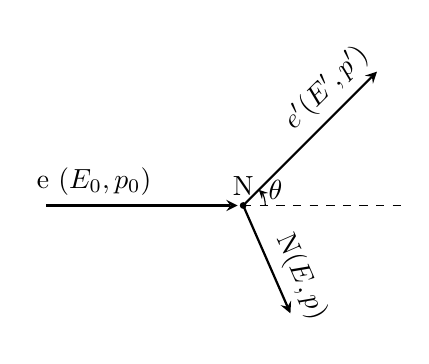
\begin{tikzpicture}
    \coordinate (N) at (0, 0);
    \coordinate (ein) at (-2.5, 0);
    \coordinate (eout) at (1.7, 1.7);
    \coordinate (p) at (0.6, -1.37);

    \filldraw[black] (N) circle (1pt);
    \node [above] at (N) {N};
    \draw[-stealth, thick] (ein) -- node [near start, above] {e ($E_0, p_0$)} ([xshift=-2pt]N);
    \draw[dashed] (N.east) -- +(2, 0);
    \draw[-stealth, thick] (N) -- node[near end, above, sloped] {$e' (E', p')$} (eout);
    \draw[-stealth, thick] (N) -- node[near end, above, sloped] {N($E, p$)} (p);
    \draw [-stealth] ([xshift=8pt]N) arc (0:45:8pt) node[right] {$\theta$};
\end{tikzpicture}
\end{center}

Energy and momentum are conserved in elastic scattering:
$$ E_0 + M = E' + E \qquad \vec{p}_0 = \vec{p}' + \vec{p} $$
where $M$ is the mass of the target nucleus.

Ignore the electron's mass, we have $E_0 \approx p_0$ and $E' \approx p'$:
\begin{equation}
    \begin{aligned}
	E^2 &= M^2 + \vec{p}^2 = M^2 + (\vec{p}_0 - \vec{p}')^2  \\
	    &= M^2 + (E_0 - E'\cos\theta)^2 + (E'\sin\theta)^2	\\
	    &= M^2 + E_0^2 + E'^2 - 2E_0E'\cos\theta	\\
	    &= (E_0 + M - E')^2
    \end{aligned}
\end{equation}

So we get:
\begin{equation}
    M(E_0 - E') = E_0E'(1-\cos\theta)   \Longrightarrow
    E' = \frac{ME_0}{M + E_0(1-\cos\theta)}
\label{eq:scattered_energy}
\end{equation}

$Q^2$ dependence on the scattering angle $\theta$ is calculated as:
\begin{equation}
    Q^2 = -q^2 = -[(E_0 - E')^2 - (\vec{p}_0 - \vec{p}')^2] = 2E_0E'(1-\cos\theta)
    \label{eq:Q2}
\end{equation}

%%%%%%%%%%%%%%%%%%%%%%%%%%%%%%%%%%%%%%%%%%%%%%%%%%%%%%%%%%%%%%%%%%%%%%%%
\section{Why Pb208 and Ca48}
\begin{figure}[!h]
    \centering
    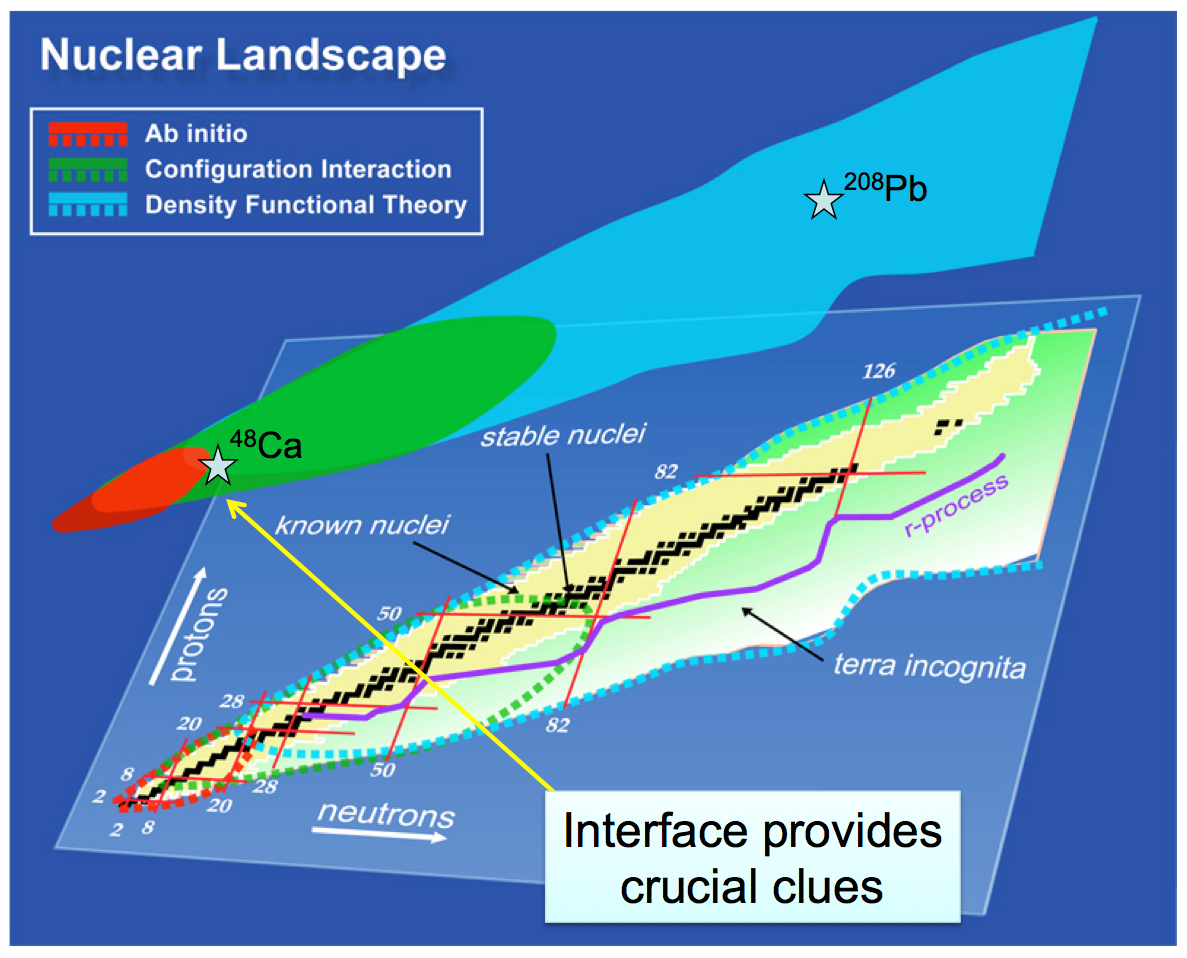
\includegraphics[width=0.5\linewidth]{Nuclear_Landscape}
    \caption{Nuclear Landscape. Figure from \cite{osti_1375323}}
    \label{fig:nuclear_landscape}
\end{figure}
As tiny as the neutron skin thickness, to obtain a relatively accurate measurement, it is
preferable to have a thicker neutron skin. Therefore, it is desirable to use a
target element with a large neutron excess. Unfortunately, most medium and heavy nuclei 
with extra neutrons are unstable due to the presence of those additional neutrons. 
Nonetheless, there are specific nuclei with certain numbers of protons and neutrons that are stable. 
These numbers are known as the magic numbers, which arise from the nucleon 
shell structure. In a magic nucleus, the outmost shell is fully filled and the 
next higher energy shell is empty. This configuration creates a barrier that makes it difficult to remove a nucleon from the closed shell.

Nuclei that posses magic numbers of both protons and neutrons are referred to 
as doubly magic nuclei. These nuclei are exceptionally stable compared to single
magic nuclei. Among the known neutron-rich doubly magic nuclei: 
${}^{10}$He, ${}^{28}$O, \Ca, ${}^{78}$Ni, ${}^{132}$Sn and \Pb, 
\Ca and \Pb are the only two stable isotopes. Therefore, they
are chosen as the target nuclei for the PREX-II and CREX.

Double magic nuclei exhibit a significant energy gap between their ground state
and the first excited state. In the case of \Ca and \Pb, the energies required
to excite them are 3.84 and 2.6~MeV respectively. 
This energy separation enables us to effectively distinguish between inelastic 
scatterings and elastic ones, thanks to the high momentum resolution of our spectrometers.

Other advantages of \Ca and \Pb include
\begin{itemize}
    \item Both nuclei are spin-0, so that we do not need to worry about the target polarization.
    \item \Pb is heavy and \Ca is moderately heavy. As discussed in the previous section, 
	elastic scattering is not exact but rather quasi-elastic. The small energy change 
	observed in the scattering is primarily due to the recoil of the target nucleus. 
	Since heavier target nuclei experience smaller recoil effects, using a heavier nucleus like \Pb improves the accuracy of our measurements for determining $Q^2$ and the scattering angle.
\end{itemize}

Finally, one more reason for the choice of \Ca: \Ca lies in the medium region of the nuclear 
landscape, as depicted in Fig.~\ref{fig:nuclear_landscape}. In comparison to \Pb, 
it is a smaller system that can be effectively studied using ab-initio methods \cite{Hagen2016}.
This allows for direct comparison to calculations based on chiral effective field theory (EFT), which is highly sensitive to three-nucleon forces. In other words, \Ca serves as a valuable probe for investigating three-nucleon forces. Additionally, \Ca is large enough to apply DFT methods. By measuring the neutron skin thickness of \Ca, we aim to provide insights that can bridge these two approaches and contribute to a deeper understanding of nuclear physics.
